\documentclass[12pt,a4paper]{report}
\usepackage[utf8]{inputenc}
\usepackage[T1]{fontenc}
\usepackage[french]{babel}
\usepackage{materialDesign}
%\ProvidesPackage{materialDesign}
\usepackage{lipsum}
\usepackage[sfdefault]{roboto}  %% Option 'sfdefault' only 
\usepackage{color}
\usepackage{xcolor}
\usepackage{tikz}
\usepackage[explicit]{titlesec}
\usepackage{enumitem}
\usepackage{afterpage}
\usepackage{caption}
\usepackage{graphicx}
\usepackage{tocvsec2}
\usepackage{fancyhdr}
\usepackage{fullpage,lmodern}
\usepackage[normalem]{ulem} % Charger le package ulem pour avoir des soulignements
\usepackage{hyperref}
\usepackage{float}
\usepackage{minted}
\usepackage[tmargin=2cm,headsep=2cm,footskip=15pt]{geometry}
\usepackage{materialDesign}

\usetikzlibrary{shadows.blur}
\usetikzlibrary{shapes.symbols}

\usePrimaryTeal
\useAccentTeal
%\useDarkTheme
\useLightTheme

% Definition des couleurs
\definecolor{accent_green}{HTML}{00E676}
\definecolor{fancystart}{HTML}{93F9B9}
\definecolor{fancyend}{HTML}{38ef7d}
% Couleurs personnalisées listes
\definecolor{azure1}{RGB}{67,233,123}
\definecolor{azure2}{RGB}{56,249,215}
% Couleurs personnalisées background
\definecolor{backgroundstart}{HTML}{232526}
\definecolor{backgroundend}{HTML}{414345}

% Texte par défaut en blanc dans le document
\color{white}

% Personnalisation des cadres (Table des matières)
\hypersetup{
    pdftitle = {Brelot Julien - Internship Report},
    %hidelinks,
    colorlinks=true,
    %linkcolor={red!20!black},
    citecolor=accent_green,
    urlcolor=accent_green,
    linkbordercolor={0 0 0},  % Supprime les bordures autour des liens
    pdfborderstyle={/S/U/W 1} % Ajoute un soulignement aux liens (U = Underline, W = Width of underline)
    % Hide links in the table of contents
}



% Personnalisation des sections
%\titleformat{\section}[block]
%    {\normalfont\Large\bfseries\color{accent_green}}
%    {\thesection}
%    {1em}
%    {}
%\titleformat{\subsection}[block]
%    {\normalfont\large\bfseries\color{accent_green}}
%    {\thesubsection}
%    {1em}
%    {\normalfont\large\bfseries\color{accent_green}{#1}}

% Numérotation des sections en chiffres romains
\renewcommand {\thesection}{\Roman{section}}
\renewcommand{\chaptername}{Partie}


%\newcommand*\sectiontitle{}
%\let\origsection\section
%\renewcommand*{\section}[2][]{%
%\ifx\setminus#1\setminus% optional argument not present?
%  \origsection{#2}%
%  \renewcommand*\sectiontitle{#2}%
%\else
%  \origsection[#1]{#2}%
%  \renewcommand*\sectiontitle{#1}%
%\fi
%}

%Formatte les titres
\titleformat{\section}[hang]
    {\Huge \bfseries\sffamily}%
    {
        \rlap{
            \color{accent}\rule[-5pt]{\textwidth}{1.2pt}
            }
        \colorbox{accent}{%
               \raisebox{0pt}[18pt][3pt]{ 
                    \makebox[40pt]{% height, width
                    \fontfamily{phv}\selectfont\color{white}{\thesection}}
                }
        }
    }%
    {10pt}%
    { \color{accent} \LARGE #1
    %
    }

% Formatte les sous titres
\titleformat{\subsection}[hang]
    {\Large \bfseries\sffamily}%
    {
        \rlap{
            \color{accent_green}\rule[-10pt]{0.93\textwidth}{1.2pt}
            }
        \colorbox{accent_green}{%
               \raisebox{0pt}[18pt][3pt]{ 
                    \makebox[20pt]{% height, width
                    \fontfamily{phv}\selectfont\color{white}{\thesubsection}}
                }
        }
    }%
    {5pt}%
    { \color{accent_green} \bfseries \large #1
    %
    }


\titlespacing*{\section}{-30pt}{3mm}{5mm}
%\titlespacing*{\subsection}{0pt}{3mm}{5mm}

%\newcommand{\sectionbreak}{\clearpage}
%\renewcommand {\thesubsection}{\arabic{subsection}.}


% Configuration du style de la table des matières
\fancypagestyle{tocstyle}{
    \fancyhf{} % Clear header and footer
    \renewcommand{\headrulewidth}{0pt} % Remove header line
    % Personnalisez ici le style de la page de la table des matières
    % Par exemple, vous pourriez ne rien ajouter ou appliquer un style plus simple.
    %\fancyfoot[C]{\thepage} % Simple page number at the center of the footer
}

% Configuration du style d'en-tête de page
\fancypagestyle{plain}{
    \fancyhf{} % Tout effacer
    \color{black}
    \renewcommand{\headrulewidth}{0pt}
    \fancyhead[C]{
        \begin{tikzpicture}[remember picture,overlay]
            \node[yshift=-1.5cm] at (current page.north west){
                \begin{tikzpicture}[remember picture, overlay]
                    % Rectangle vert en arrière-plan sans le dégradé
                    \draw[fill=accent,blur shadow={shadow blur steps=10}] (0,0) rectangle (\paperwidth,2cm);
                    % Dégradé dans le rectangle avec coins arrondis
                    \node[anchor=center,xshift=.5\paperwidth,yshift=0.8cm, rectangle,rounded corners,inner sep=9pt,left color=fancystart, right color=fancyend, blur shadow={shadow blur steps=10}]
                        {\color{black} \Large \leftmark}; % \thesection -
                \end{tikzpicture}
            };
        \end{tikzpicture}
    }

    % Configuration du style de pied de page (numéro de page)
    %\pagestyle{fancy}
    %\fancyhf{} % Clear all header and footer fields
    %\renewcommand{\headrulewidth}{0pt} % Remove header line
    \fancyfoot{%
    \begin{tikzpicture}[remember picture, overlay]
        \fill[left color=azure1,right color=azure2] (current page.south) ++(0em,2em) circle (1.5em);
        \node[anchor=south,text=textAccent, yshift=1.3em] at (current page.south) { \hyperlink{toc}{\bf \thepage}};
    \end{tikzpicture}%
    }
}

\setlength{\headheight}{15pt} % Avoids fancyhdr warning

% Personnalisation des listes
\setlist[enumerate,1]{label=\textcolor{accent}{\textbullet}}
\setlist[itemize,1]{label=\textcolor{accent}{\Large $\bullet$}}



\begin{document}

% Ajouter une cible pour le lien de retour à la table des matières
\addtocontents{toc}{\protect\hypertarget{toc}{}}

% Page de garde
%\pagecolor{backgroundstart}
\begin{titlepage}

    % Dégradé en fond 
    \begin{tikzpicture}[remember picture,overlay]
        \shade[top color=backgroundstart,bottom color=backgroundend] (current page.south west) rectangle ++(\paperwidth,\paperheight);
    \end{tikzpicture}

    % Rectangle en arrière-plan (vert en haut)
    \begin{tikzpicture}[remember picture,overlay]
        \fill[fill=accent] (current page.north west) rectangle ++(\paperwidth,-2cm);
    \end{tikzpicture}
    
    % Rectangle en arrière-plan (vert en bas)
    \begin{tikzpicture}[remember picture,overlay]
        \fill[fill=accent] (current page.south west) rectangle ++(\paperwidth,2cm);
    \end{tikzpicture}
    
    \vfill % Adds vertical space, pushing content down to the center

    % Titre du rapport
    \begin{center}
        {\Huge \bfserie Rapport de Comparaison des Performances
        entre MySQL et MongoDB }
        \par}
    \end{center}
    
    \vspace{1cm} % Adds a little space between title and author section
    
    % Auteur et affiliation
    \begin{center}
        {\LARGE Brelot Julien\par}
    \end{center}

    \vspace{1.5cm} % Adds space between author info and logos

    % Logos
    \begin{center}
        \begin{minipage}{0.45\textwidth}
            
\includegraphics[width=\textwidth]{images/logo-tps.png}
        \end{minipage}
        \hfill
        \begin{minipage}{0.45\textwidth}
            
\includegraphics[width=\textwidth]{images/logo_imt.png}
        \end{minipage}
    \end{center}
    
    \vspace{1.5cm} % Adds space between logos and VTEC logo

    
    \vfill % Adds vertical space, pushing content up to the center
    
\end{titlepage}
%\setcounter{section}{31} 

\thispagestyle{tocstyle}
\tableofcontents % Table des matières
\clearpage % Passer à la page suivante
\listoffigures
\clearpage

\pagestyle{plain} % Style de page pour le contenu


\chapter{Introduction}

\begin{card}
Ce rapport présente une étude comparative des performances entre MySQL et MongoDB, deux systèmes de gestion de bases de données (SGBD) très utilisés, en mettant l'accent sur les opérations CRUD (Create, Read, Update, Delete).\newline
L'objectif est de tester différentes configurations et scénarios d'utilisation pour analyser l'impact des index, de la réplication, et de la fragmentation sur les performances.\newline
La structure des tests, ainsi que les résultats obtenus, sont décrits en détail.
\end{card}

\chapter{Contexte et Objectifs}

\section{Systèmes Comparés}


    \subsection{MongoDB}
    \begin{card}
        MongoDB est un SGBD NoSQL orienté documents. 
        Contrairement aux bases relationnelles, MongoDB stocke les données sous forme de documents JSON ou BSON, offrant une grande flexibilité structurelle. Ses caractéristiques principales incluent :

        \begin{itemize}
            \item \textbf{Stockage orienté documents} : Les données sont regroupées en collections, chaque document étant un objet JSON avec une structure flexible.
            \item \textbf{Requêtes riches} : MongoDB prend en charge des requêtes complexes incluant des opérations d'agrégation et des jointures.
            \item \textbf{Scalabilité horizontale} : Avec la fragmentation (sharding), les données peuvent être réparties sur plusieurs nœuds.
            \item \textbf{Réplication} : MongoDB utilise des Replica Sets pour garantir la haute disponibilité et la tolérance aux pannes.
            \item \textbf{Indexation avancée} : MongoDB offre un support pour les index secondaires et composites afin d'optimiser les performances des requêtes.
        \end{itemize}
    \end{card}

    \subsection{MySQL}
        \begin{card}
            MySQL est un SGBD relationnel open-source largement utilisé dans les applications web et les systèmes d'information. 
            Ses caractéristiques principales incluent :
            \begin{itemize}
                \item \textbf{Modèle relationnel} : Les données sont stockées dans des tables avec des relations définies par des clés étrangères.
                \item \textbf{Transactions ACID} : MySQL garantit l'atomicité, la cohérence, l'isolation et la durabilité des transactions.
                \item \textbf{Indexation} : Prise en charge d'index pour optimiser les performances des requêtes.
                \item \textbf{Réplication} : MySQL utilise un modèle maître-esclave pour répliquer les données entre plusieurs serveurs.
                \item \textbf{Clusterisation} : MySQL Cluster permet de distribuer les données sur plusieurs nœuds
            \end{itemize}
        \end{card}
        
\section{Étude des aspects de MongoDB}

    \subsection{Comparaison des Performances des Requêtes}
        \begin{card}
            MongoDB se distingue des bases relationnelles comme MySQL par sa capacité à exécuter des requêtes sur des données semi-structurées et non structurées. 
            La comparaison des performances des requêtes révèle :
            \begin{itemize}
                \item MongoDB excelle dans les scénarios où les données sont semi-structurées ou nécessitent une mise à jour fréquente de leur structure.
                \item MySQL, en revanche, est plus performant pour les requêtes transactionnelles complexes grâce à son moteur ACID robuste.
                \item Les schémas flexibles de MongoDB permettent une évolutivité plus facile pour les applications en croissance.
                \item La mise à l'échelle horizontale de MongoDB via la fragmentation (sharding) est un avantage pour les applications nécessitant une haute disponibilité et une distribution des données.
                \item Tolérance aux pannes : MongoDB offre une haute disponibilité des données grâce à la réplication automatique et aux élections de nœuds primaires.
                \item Les performances de lecture/écriture peuvent être optimisées en configurant les politiques de réplication et de fragmentation.
            \end{itemize}
        \end{card}

    \subsection{Performances avec et sans Indexation}

        \begin{card}
            L'indexation est un facteur clé des performances :
            \begin{itemize}
                \item \textbf{MongoDB sans indexation} : Les requêtes nécessitent un balayage complet des documents, ce qui ralentit considérablement les performances.
                \item \textbf{MongoDB avec indexation} : Les performances des lectures augmentent considérablement grâce à la réduction du nombre de documents scannés.
                \item \textbf{MySQL avec indexation} : Étant donné sa nature relationnelle, MySQL exploite efficacement les index pour optimiser les lectures et écritures.
            \end{itemize}
        \end{card}

    \subsection{Réplication et Fragmentation}
        \begin{card}
            La réplication et la fragmentation influencent directement les performances et la tolérance aux pannes.
        
            \paragraph{Réplication dans MongoDB :}
            \begin{itemize}
                \item \textbf{Réplication primaire-secondaire} : Permet une haute disponibilité des données. Les écritures se font uniquement sur le nœud primaire, tandis que les lectures peuvent être réparties sur les nœuds secondaires.
                \item \textbf{Élections automatiques} : En cas de panne du nœud primaire, un nouveau primaire est élu parmi les secondaires, garantissant une continuité de service.
                \item \textbf{Impact sur les performances} : La latence d'écriture augmente avec un \texttt{write concern} élevé, car l'écriture doit être confirmée par plusieurs nœuds.
            \end{itemize}

            \paragraph{Fragmentation dans MongoDB :}

            \begin{itemize}
                \item \textbf{Distribution des données} : Les documents sont répartis entre plusieurs shards, permettant de gérer efficacement de grandes volumétries.
                \item \textbf{Impact sur les performances} : La fragmentation améliore les temps de réponse pour les lectures et écritures parallèles, mais peut augmenter la complexité des requêtes agrégées.
            \end{itemize}
        \end{card}



\chapter{Structure des Tests}

\section{Architecture MongoDB}

Pour les tests de performance, nous avons utilisé trois architectures MongoDB différentes : Standalone, Replica Set, et Sharded Cluster.
Pour MySQL, nous avons testé deux configurations : Standalone et Cluster. 
Ceci afin d'estimer l'impact du choix de l'architecture sur les performances des opérations CRUD.

    \subsection{Architecture avec serveur unique : Standalone}

        Un seul serveur MongoDB.
        
        \begin{figure}[H]
            \centering
            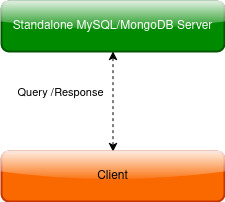
\includegraphics[width=0.8\textwidth]{architectures/Standalone.jpg}
            \caption{Architecture Standalone.}
            \label{fig:standalone}
        \end{figure}

    \subsection{Architecture avec réplications : Replica Set}

        Un Replica Set avec un nœud primaire et deux nœuds secondaires.
        \begin{figure}[H]
            \centering
            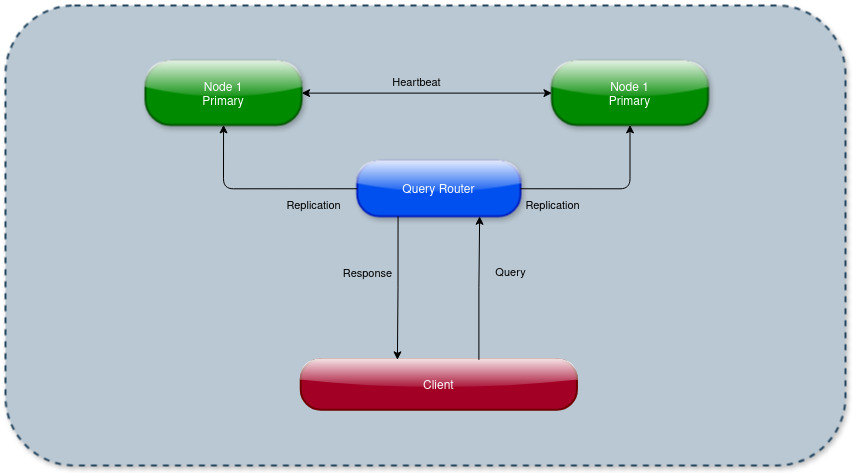
\includegraphics[width=0.8\textwidth]{architectures/MongoDBReplica.jpg}
            \caption{Architecture Replica Set.}
            \label{fig:mongo-replica-set}
        \end{figure}

    \subsection{Architecture Fragmentée : shards}
        Un cluster avec trois Serveurs de configuration, un Query router, et deux shards constitués chacun de deux nœuds.
        On aurait pu mettre 3 noeuds par shard, mais pour des raisons de ressources, on a opté pour 2.

        \begin{figure}
            \centering
            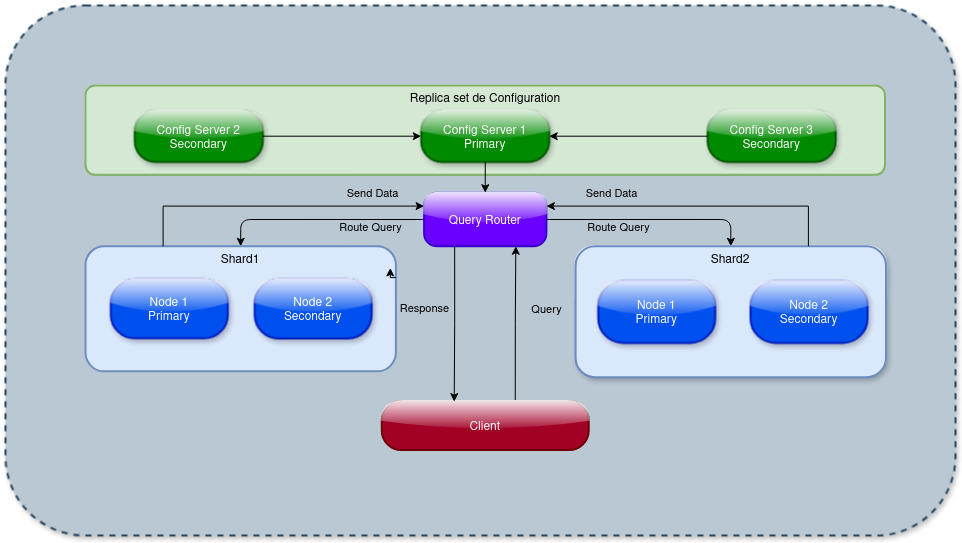
\includegraphics[width=0.8\textwidth]{architectures/MongoDBShards.jpg}
            \caption{Architecture Sharded Cluster de MongoDB.}
            \label{fig:mongo-sharded-cluster}
        \end{figure}

\section{Architecture MySQL}

    \subsection{Architecture avec serveur unique : Standalone}

        Un serveur MySQL simple.
        Voir la figure \ref{fig:standalone}.

    \subsection{Architecture Distribuée : Cluster}

        Architecture MySQL-NDB avec :
        \begin{itemize}
            \item Un gestionnaire (manager).
            \item Deux nœuds de données.
            \item Un noeud SQL.
        \end{itemize}

        \begin{figure}[H]
            \centering
            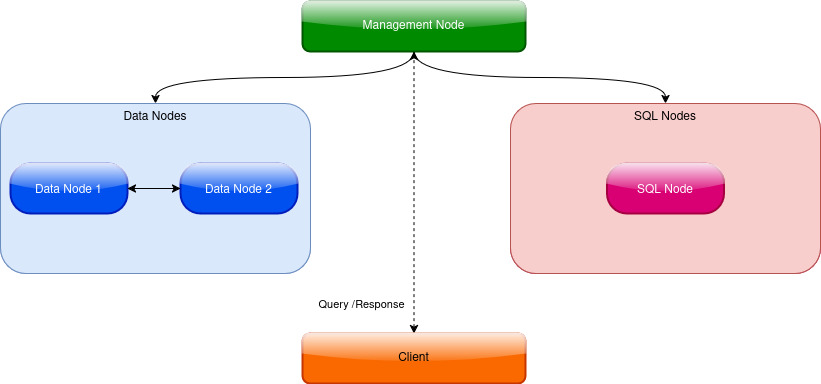
\includegraphics[width=0.8\textwidth]{architectures/MySQLCluster.jpg}
            \caption{Architecture MySQL Cluster.}
            \label{fig:mysql-cluster}
        \end{figure}


\section{Description des Tests}

    \subsection{Contexte}
        \begin{card}
            Avant l'execution des tests, il est nécessaire de générer les données de test. \\
            Cela est possible grâce au script Python \textit{generate\_data.py} qui génère des données aléatoires pour les tests de performance. \\
            Ce script repose sur l'utilisation du module \href{https://faker.readthedocs.io}{Faker} pour générer des données aléatoires pour les tests. \\
            Une graine  a été employée afin d'avoir des résultats reproductibles. \\
            Pour MongoDB et MySQL respectivement, Les tests de performance sont réalisés en utilisant des scripts Python (\textit{mongodb.py}, \textit{mysql.py}) et les modules clients \href{https://pymongo.readthedocs.io}{pymongo}, \href{https://pymysql.readthedocs.io}{pymysql}. \\
            Ces scripts effectuent des opérations et mesurent les temps d'execution des opérations CRUD sur les bases de données. \\
            Notons que le module \href{https://pymongo.readthedocs.io}{pymongo} intègre un sous module pour monitorer les temps d'execution des requêtes pour les tests, reposant sur les retours de MongoDB. \\
            En revanche, pour MySQL, les temps d'execution sont mesurés en utilisant le module en local en mesurant l'intervalle de temps entre l'envoi et la réception des requêtes. \\
            Ainsi, les tests dépendent également en partie de la latence réseau, néanmoins, le docker compose \textit{docker-compose.yml} permet de déployer des serveurs en local et de s'affranchir de cette limite. \\
            Enfin, le module \href{https://matplotlib.org}{matplotlib} est utilisé pour générer des graphiques à partir des résultats des tests.
        \end{card}

    \subsection{Principe des tests}
        \begin{card}
            Il y a fondamentalent 2 types de tests :
            \begin{itemize}
                \item Tests globaux : \texit{N} Opérations CRUD succesives sur l'ensemble des données.
                \item Tests avec variation de quantité de données initiales : Opérations CRUD données avec variation du nombre de données initiales.
            \end{itemize}

            Les tests globaux visent à mesurer les statistiques globales des opérations succesives de \textit{N} insertions, \textit{N} mises à jour,\textit{N} lectures, puis \textit{N} suppression de données. \\
            Les tests avec variation de quantité de données initiales insèrent en premier lieu, un nombre $ x_n $  de données initiales. \\
            Ensuite, on mesure le temps d'execution d'une operation d'insertion, puis de mise à jour, de lecture et de suppression de données. \\
            On répète ces opérations \textit{n} fois pour des quantités de données initiales $ x_n $ différentes entre 0 et \textit{N}. \\

            Dès lors, on s'intéresse à la différence de performance entre pération CRUD avec des données uniques et des données multiples. \\
            Par exemple, on regarde la différence entre 10 insertions de 10 données distinctes une par une, et l'insertion de 10 données en une seule fois. \\
            Ainsi, ces tests effectueront  $ \frac{N}{n\_donnees\_par\_operation} $ opérations CRUD. \\

            Finalement, on voudrait mesurer l'impact de l'indexation sur les performances des opérations CRUD. \\

            On fera donc au total 8 tests par infrastructure de base de données, soit 24 tests au total. \\
            En effet, on réplique les 2 types de tests pour des opérations uniques et des opérations multiples, et cela avec et sans indexation. \\
            \end{card}

   \subsection{Paramètres des tests}
        \begin{card}
            Les paramètres de la génération des données et des tests est configurable via le fichier \textit{.env.py}.
            On peut configurer : 
            \begin{itemize}
                \item \texttt{NUM\_RECORDS} : Nombre de données à générer.
                \item \texttt{NUM\_RECORDS\_PER\_MANY} : Nombre de données à intégrer dans une seule requête. Exemple : insertion de 10 objets en une seule requête.
                \item \texttt{NB\_MEASUREMENTS} : Nombre de mesures à réaliser pour les tests avec variation de quantité de données initiales.
                \item Les adresses et les ports des serveurs MongoDB et MySQL.
            \begin{itemize}

            Les valeurs utilisées dans les tests et amenant aux résultats des tests sont les suivantes :
            \begin{itemize}
                \item \texttt{NUM\_RECORDS} = 25000
                \item \texttt{NUM\_RECORDS\_PER\_MANY} = 25
                \item \texttt{NB\_MEASUREMENTS} = 1000
            \end{itemize}
        \end{card}

    \subsection{Structure des Données}
        \begin{card} 
            Afin de tenter de mesurer les performances des bases de données, sans favoriser l'une ou l'autre, les données générées sont les mêmes pour les deux bases de données. \\
            Elles sont génériques et construites pour éviter d'exploiter des fonctionnalités spécifiques à l'une ou l'autre base de données. \\
            Elles intégrent différents types de données, tels que des chaînes de caractères, des dates, des nombres entiers et des nombres flottants. \\

            Ainsi, La table/collection "test" utilisée pour les tests, regroupe des données avec la structure suivante :
            \begin{itemize}
                \item \textbf{id} : Identifiant unique (UUID ou auto-incrément pour MySQL, ObjectId pour MongoDB).
                \item \textbf{title} : Titre du livre (String).
                \item \textbf{author} : Auteur du livre (String).
                \item \textbf{published\_date} : Date de publication (Date).
                \item \textbf{genre} : Genre du livre (String).
                \item \textbf{price} : Prix du livre (Float).
                \item \textbf{copies\_sold} : Nombre d'exemplaires vendus (Integer).
                \item \textbf{ran} : Champ aléatoire pour les tests entre 0 et $\texttt{num\_records\_per\_many} - 1$ (Integer).
            \end{itemize}
        
            Ce qui donne pour MySQL :
        
            \begin{verbatim}
                CREATE TABLE test (
                    id INT ,
                    title VARCHAR(255),
                    author VARCHAR(255),
                    published_date DATE,
                    genre VARCHAR(255),
                    price FLOAT,
                    copies_sold INT,
                    ran INT
                );
            \end{verbatim}
        \end{card}



\chapter{Résultats et Analyses pour MongoDB}

\section{MongoDB Standalone}

    \subsection{Performances des Opérations uniques}

        \subsubsection{Distribution des performances des opérations CRUD uniques}
        \begin{figure}[H]
            \centering
            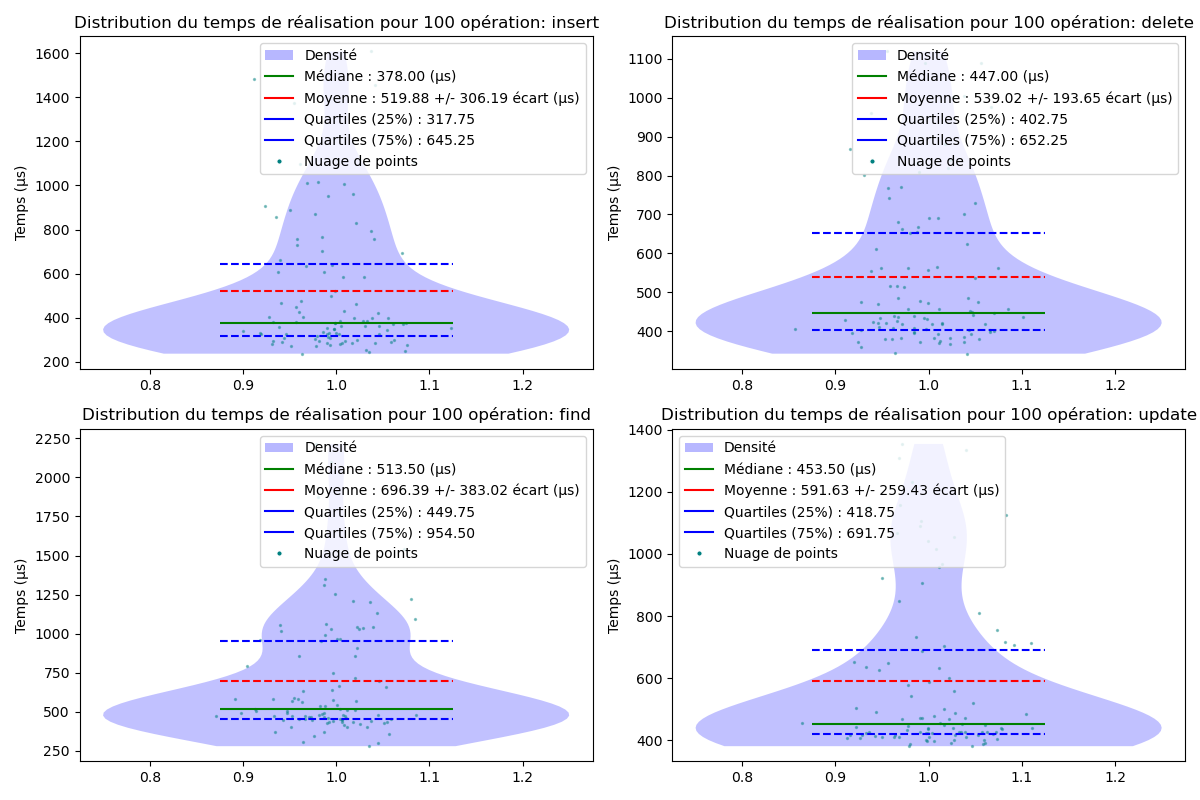
\includegraphics[width=0.8\textwidth]{../plots/MongoDB/standalone/global_test_one.png}
            \caption{Distribution des performances des opérations CRUD uniques.}
            \label{fig:mongo_standalone_global_one}
        \end{figure}
      
        \subsubsection{Performances des Opérations uniques selon la quantitée de données dans la base}
        \begin{figure}[H]
            \centering
            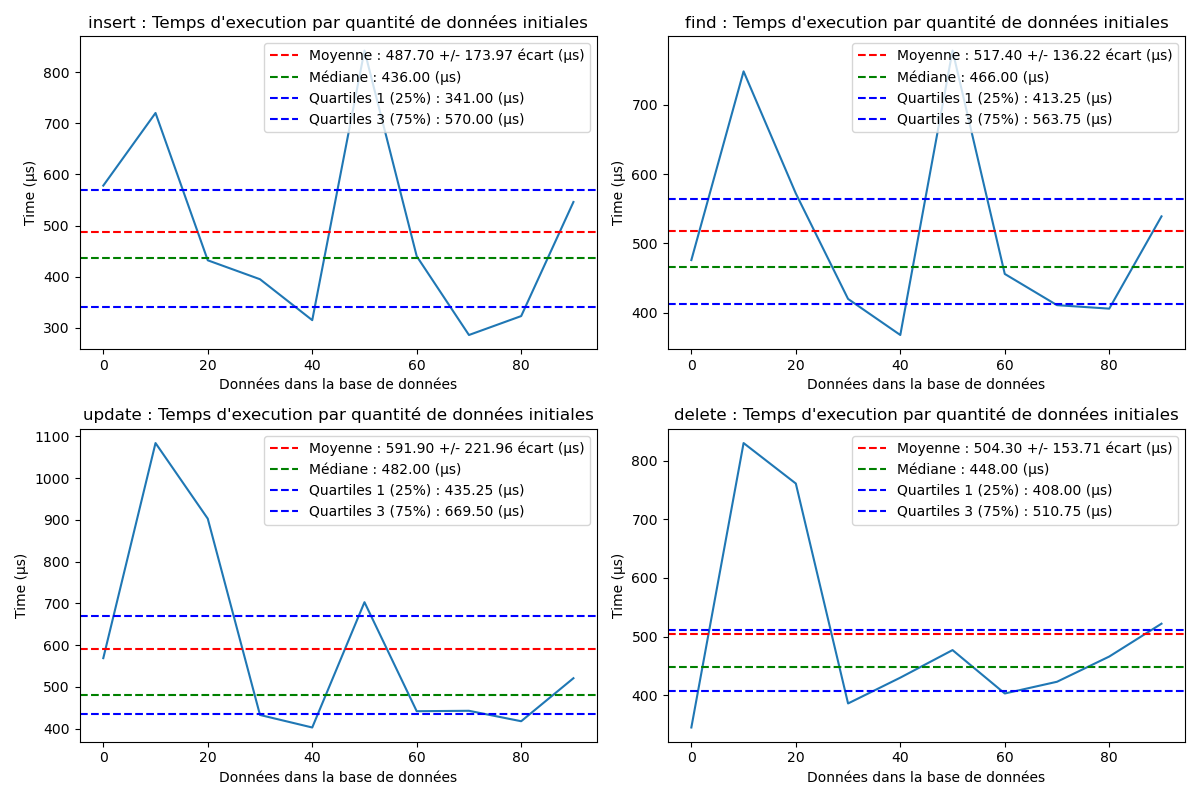
\includegraphics[width=0.8\textwidth]{../plots/MongoDB/standalone/test_one_various_data.png}
            \caption{Performances des opérations CRUD uniques selon la quantitée de données dans la base.}
            \label{fig:mongo_standalone_one_various}
        \end{figure}

        % Petite Analyse des résultats
        \begin{card}
            Les résultats montrent que l'insertion des données se fait en temps quasiment constant, \\
            tandis que les autres opérations évoluent linéairement avec la quantité de données.     \\
            Cela  reflète une augmentation des coûts de recherche dans les collections non indexées.\\
        \end{card}

    \subsection{Performances des Opérations avec données multiples}

        \begin{figure}[H]
            \centering
            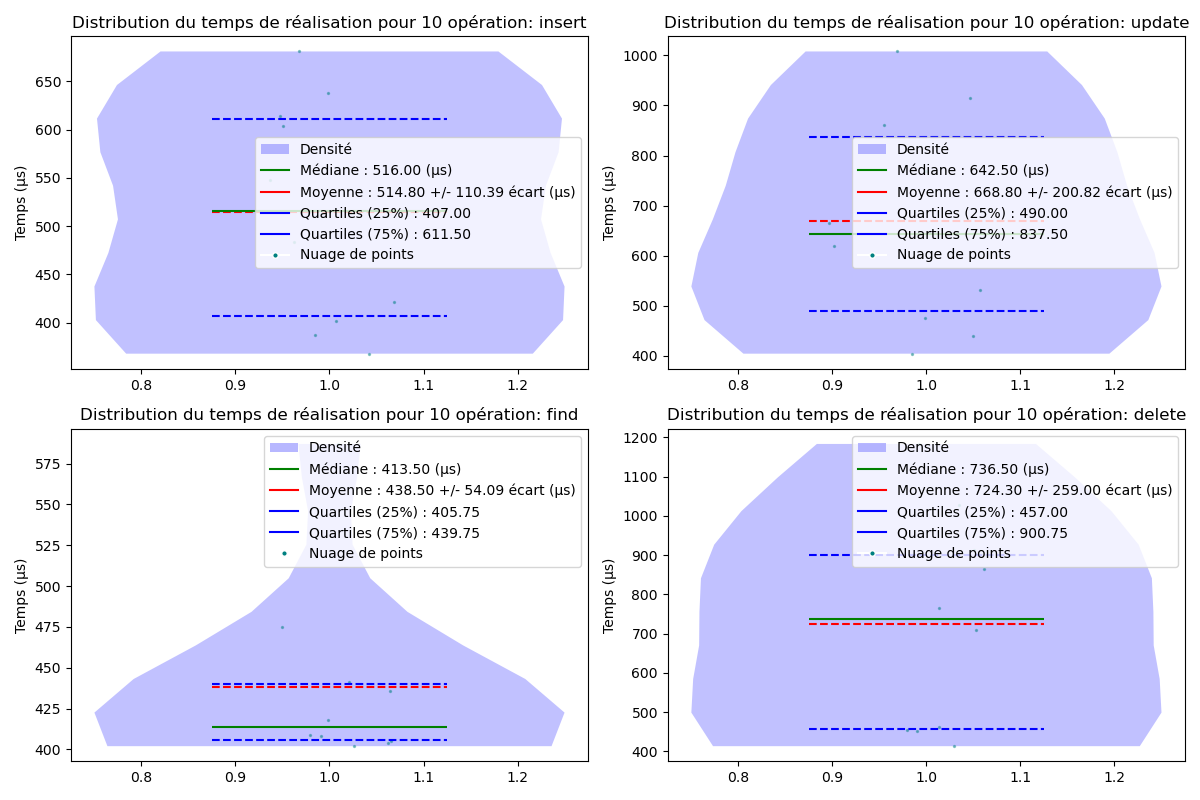
\includegraphics[width=0.8\textwidth]{../plots/MongoDB/standalone/global_test_many.png}
            \caption{Distribution des performances des opérations CRUD multiples.}
            \label{fig:mongo_standalone_global_many}
        \end{figure}

        \begin{figure}[H]
            \centering
            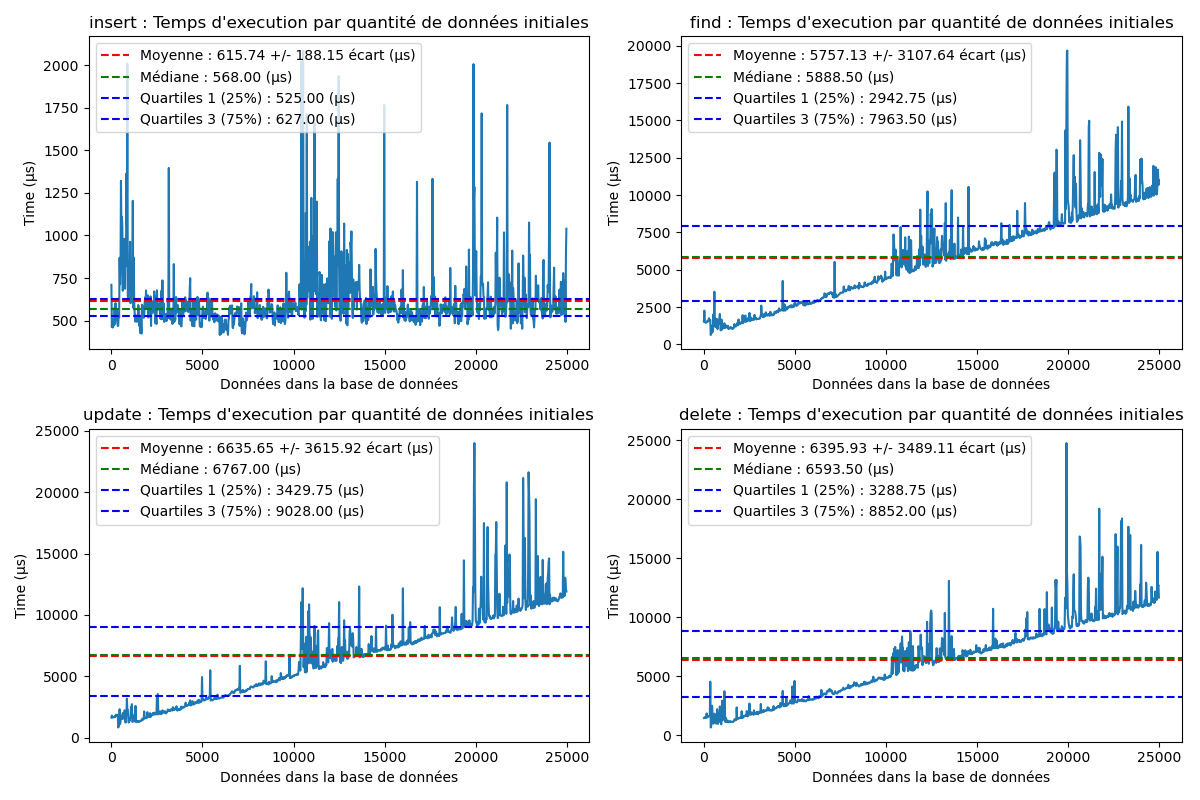
\includegraphics[width=0.8\textwidth]{../plots/MongoDB/standalone/test_many_various_data.png}
            \caption{Performances des opérations CRUD multiples selon la quantitée de données dans la base.}
            \label{fig:mongo_standalone_many_various}
        \end{figure}

        \begin{card}
            Les résultats sont semblables et assez proches numériquement de ceux des opérations uniques. \\
            On remarque néanmoins que les temps d'execution sont plus longs pour les opérations multiples, ce qui est attendu. \\
            La différence n'est certainement pas assez notable car trop peu de données sont opérer en simultanées (25 données à la fois) pour que cela ait un impact significatif. \\
            néanmoins, on remarque que les temps d'execution augmente plus ainsi que le variance pour la modification de données. \\
            Cependant, rapporté au nombre de données sur lequel on opére en une fois et au temps proche de l'opération unique,  \\
            on peut en conclure que les opérations multiples sont plus intéressantes que les opérations uniques dans le cas sans indexation.
        \end{card}

        \subsection{Indexation}
        
            \subsubsection{Performances des Opérations uniques}

                \begin{figure}[H]
                    \centering
                    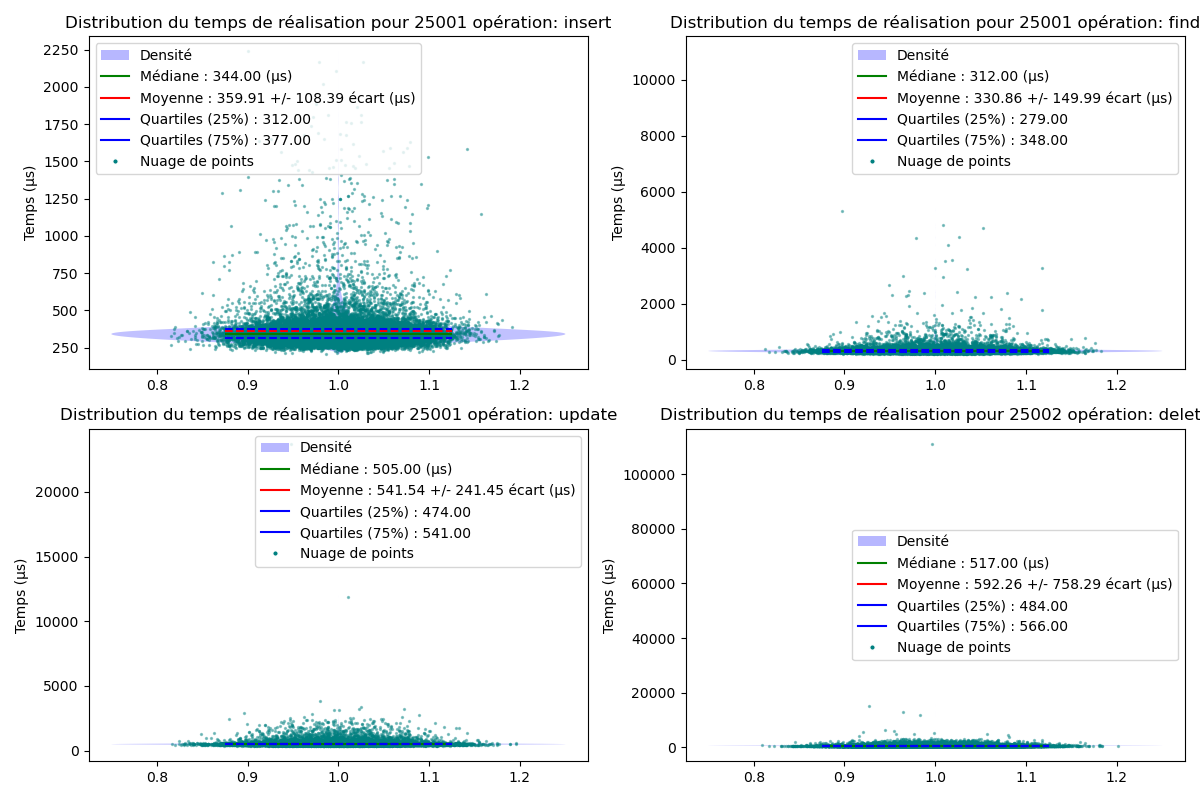
\includegraphics[width=0.8\textwidth]{../plots/MongoDB/standalone_indexed/global_test_one.png}
                    \caption{Distribution des performances des opérations CRUD uniques.}
                    \label{fig:mongo_standalone_global_one_indexed}
                \end{figure}

                \begin{figure}[H]
                    \centering
                    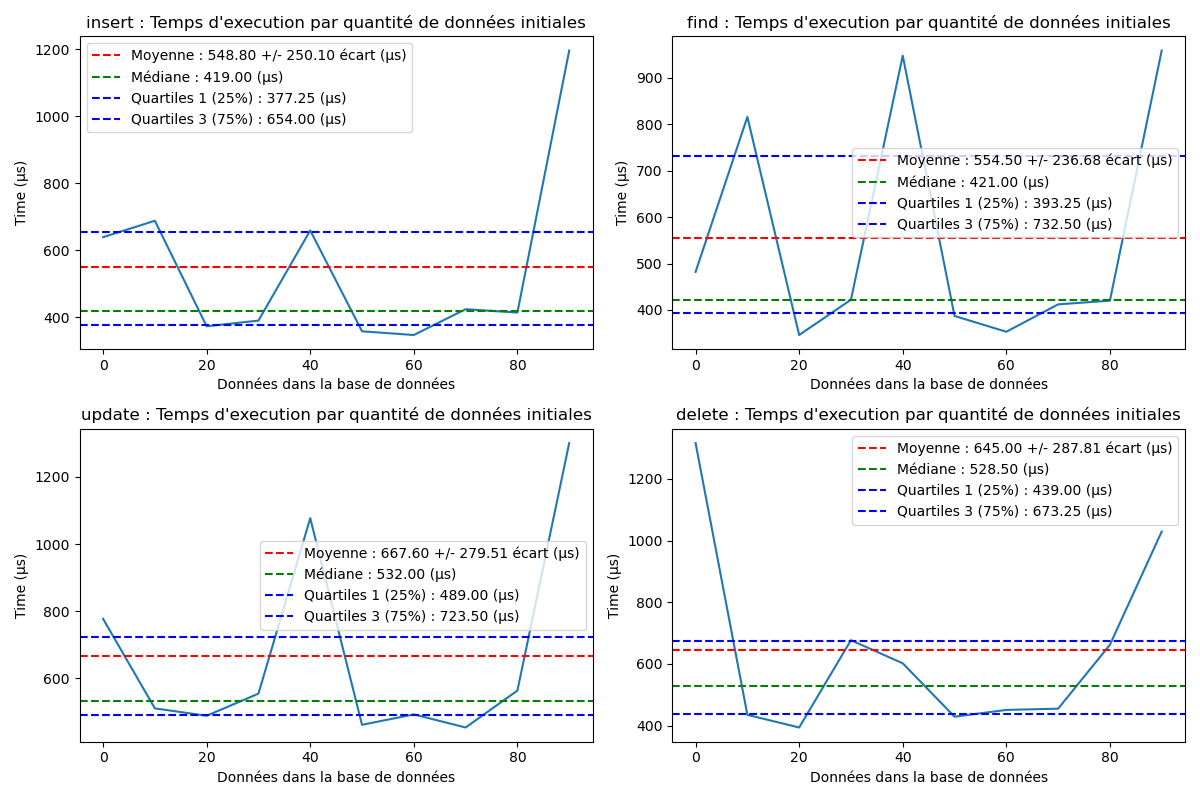
\includegraphics[width=0.8\textwidth]{../plots/MongoDB/standalone_indexed/test_one_various_data.png}
                    \caption{Performances des opérations CRUD uniques selon la quantitée de données dans la base.}
                    \label{fig:mongo_standalone_global_one_various_indexed}
                \end{figure}

                \begin{card}
                    On observe ici une nette amélioration des performances pour les opérations de lecture et de mise à jour, et suppression (près de 10 fois plus rapide en moyenne).\\
                    En ce qui conceren l'insertion, les performances sont proches mais légèrement plus lentes. \\
                    L'évolution n'est plus linéaire, ce qui montre l'efficacité de l'indexation, les opérations sont faites presques en temps constant en moyenne. \\
                    On observe simplement des pics de variations, due à l'indexation. Néamoins l'écart type reste comparable au cas sans indexation. 
                \end{card}

            \subsubsection{Performances des Opérations avec données multiples}

                \begin{figure}[H]
                    \centering
                    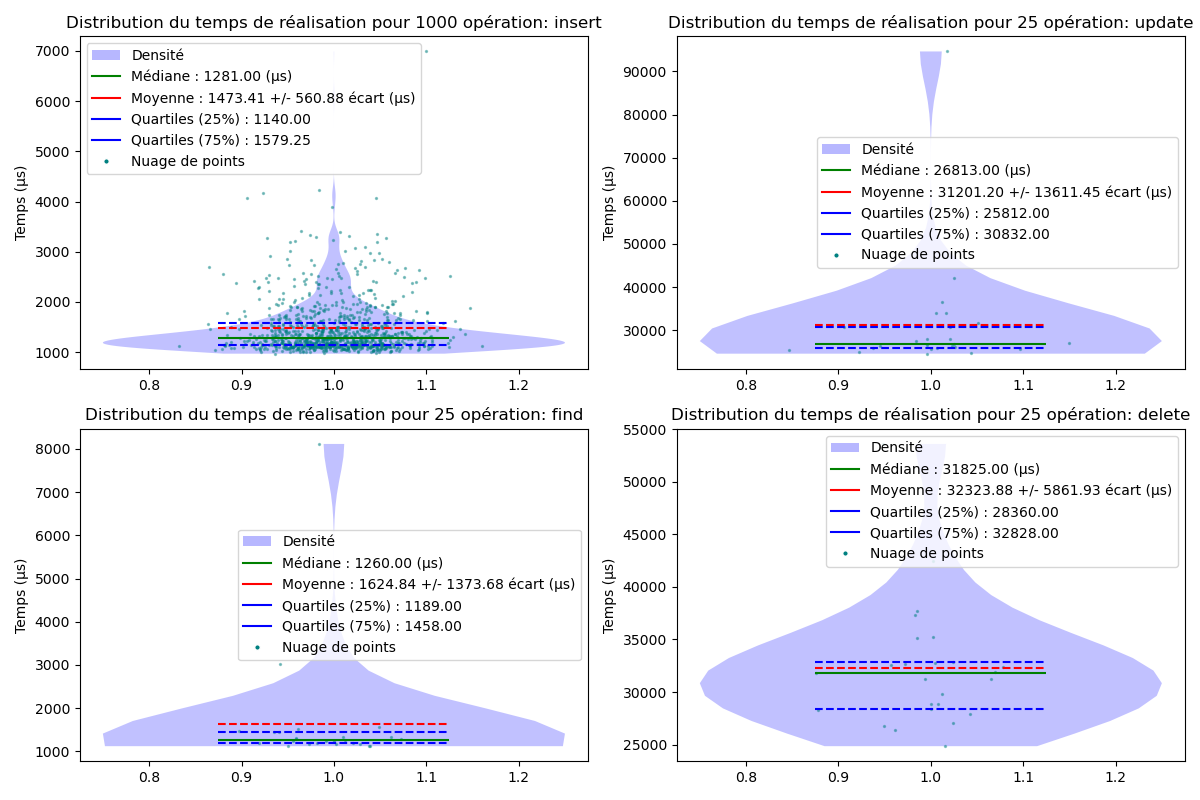
\includegraphics[width=0.8\textwidth]{../plots/MongoDB/standalone_indexed/global_test_many.png}
                    \caption{Distribution des performances des opérations CRUD multiples.}
                    \label{fig:mongo_standalone_global_many_indexed}
                \end{figure}

                \begin{figure}[H]
                    \centering
                    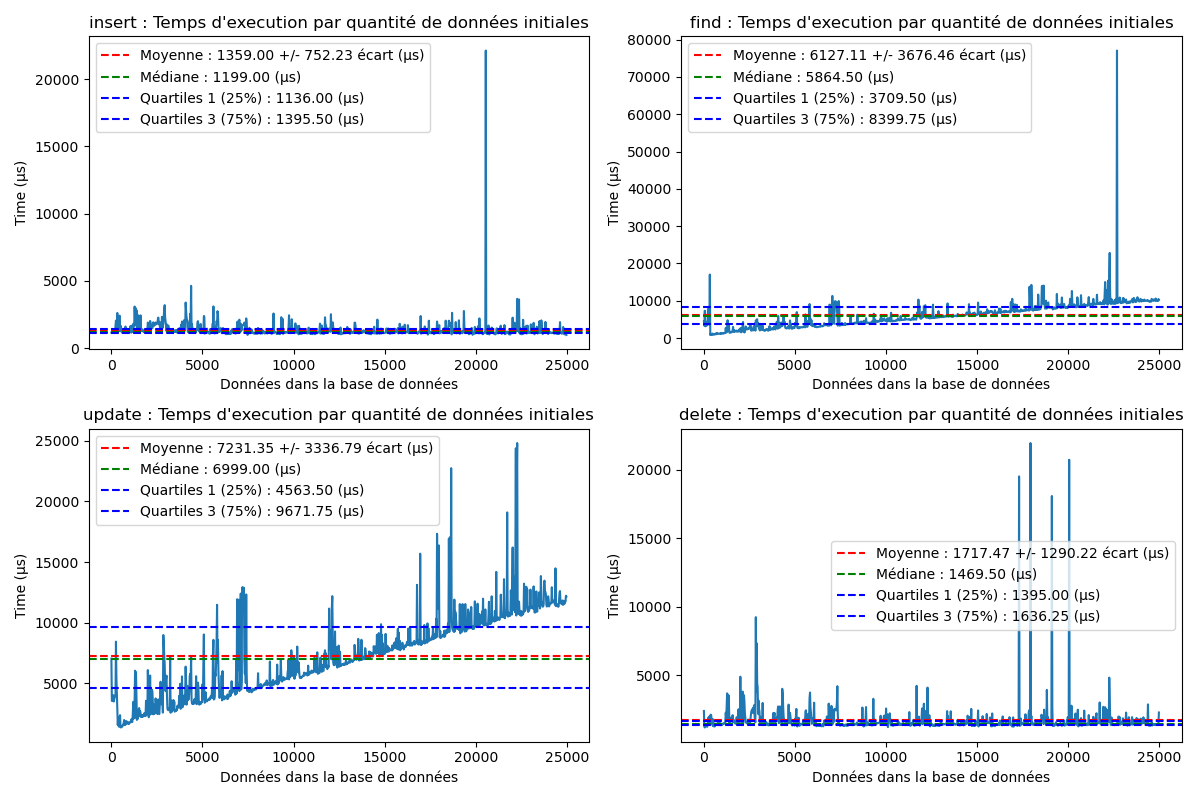
\includegraphics[width=0.8\textwidth]{../plots/MongoDB/standalone_indexed/test_many_various_data.png}
                    \caption{Performances des opérations CRUD multiples selon la quantitée de données dans la base.}
                    \label{fig:mongo_standalone_global_many_various_indexed}
                \end{figure}

                \begin{card}
                    Ici, les observations se tiennent pour l'insertion et la supression. \\
                    En revanche, on observe une évolution linéaire légèrement coefficienté qui semble s'amortir pour la modification et la lecture. \\
                    Les performances affichées sembelent bien moins bonnes que pour les opérations uniques, mais rapporté au nombre de données sur lequel on opére (25) en une fois, \\
                    on peut en conclure que les opérations multiples reste plus intéressantes que les opérations uniques dans le cas avec indexation.
                    Néanmoins, il  faudrait certainement trouver un point d'équilibre ( le nombre de données sur lequel on opère en une fois) pour optimiser les performances. \\
                \end{card}


\section{Réplication}

    \subsection{Performances des Opérations uniques}

        \begin{figure}[H]
            \centering
            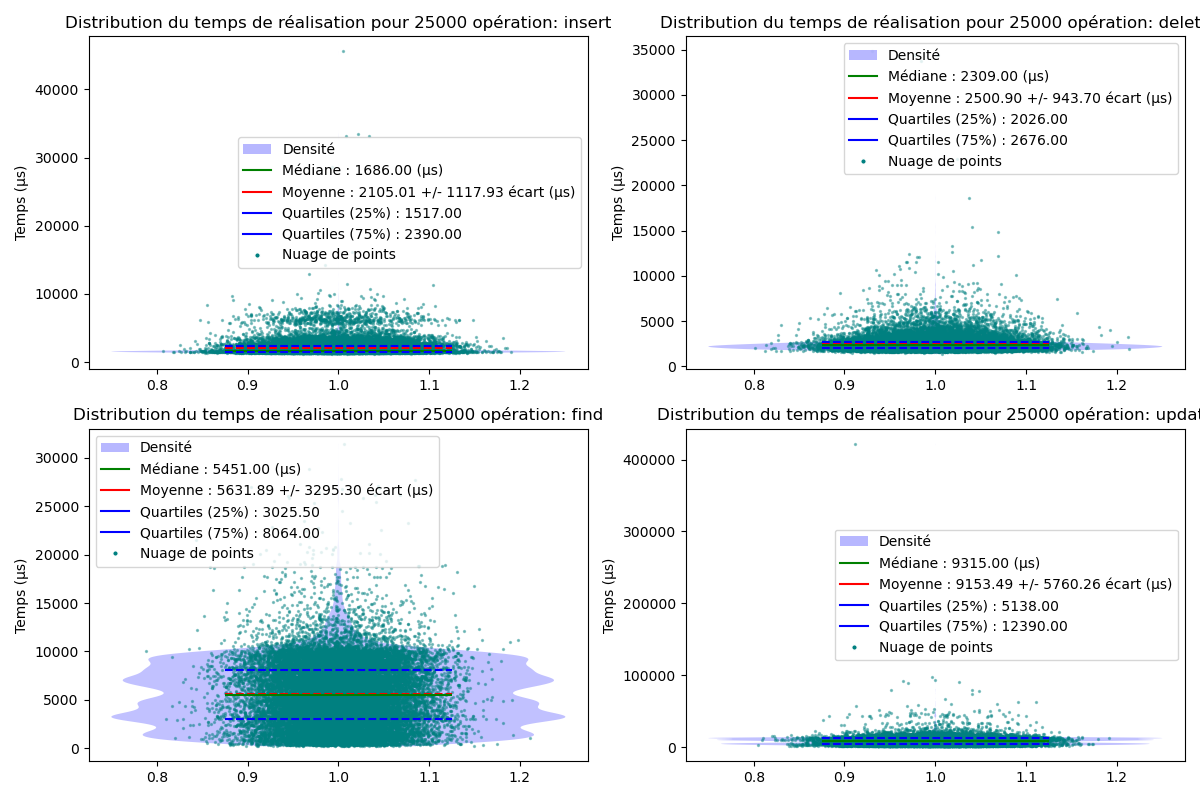
\includegraphics[width=0.8\textwidth]{../plots/MongoDB/replica_set/global_test_one.png}
            \caption{Distribution des performances des opérations CRUD uniques.}
            \label{fig:mongo_replica_global_one}
        \end{figure}

        \begin{figure}[H]
            \centering
            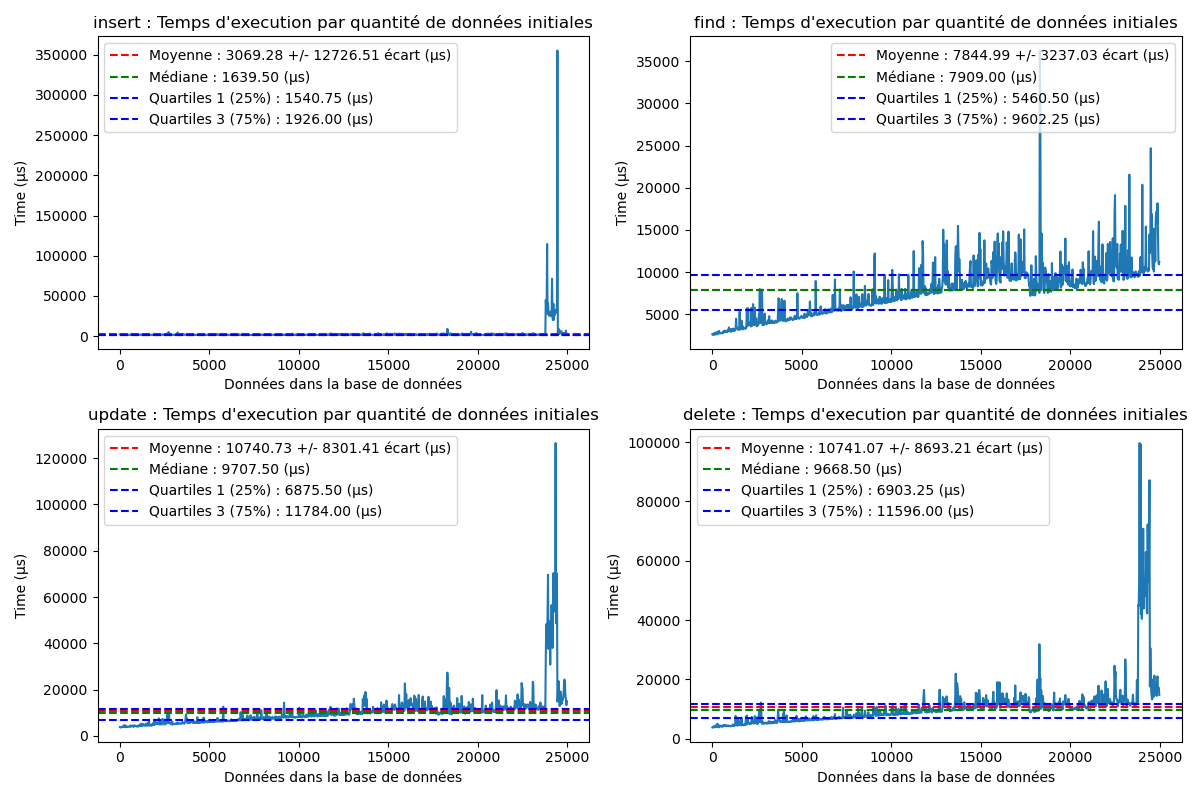
\includegraphics[width=0.8\textwidth]{../plots/MongoDB/replica_set/test_one_various_data.png}
            \caption{Performances des opérations CRUD uniques selon la quantitée de données dans la base.}
            \label{fig:mongo_replica_one_various}
        \end{figure}

    \subsection{Performances des Opérations avec données multiples}

        \begin{figure}[H]
            \centering
            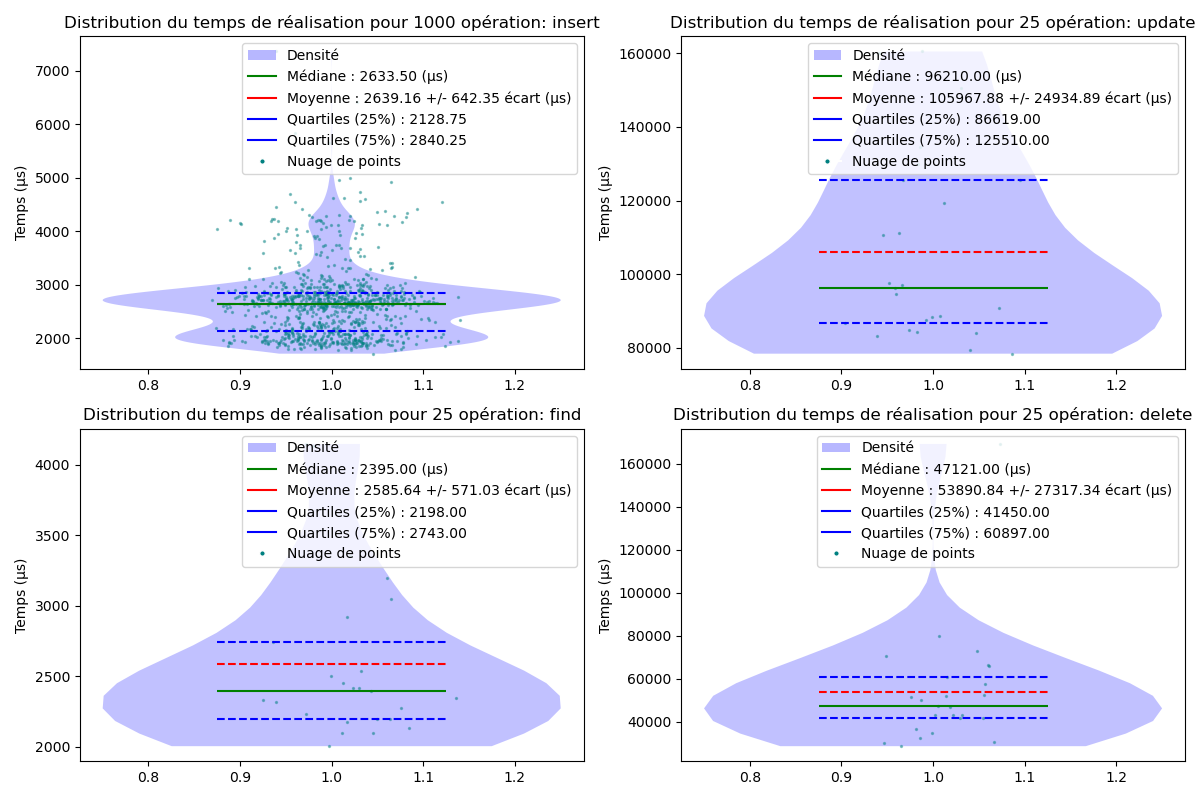
\includegraphics[width=0.8\textwidth]{../plots/MongoDB/replica_set/global_test_many.png}
            \caption{Distribution des performances des opérations CRUD multiples.}
            \label{fig:mongo_replica_global_many}
        \end{figure}

        \begin{figure}[H]
            \centering
            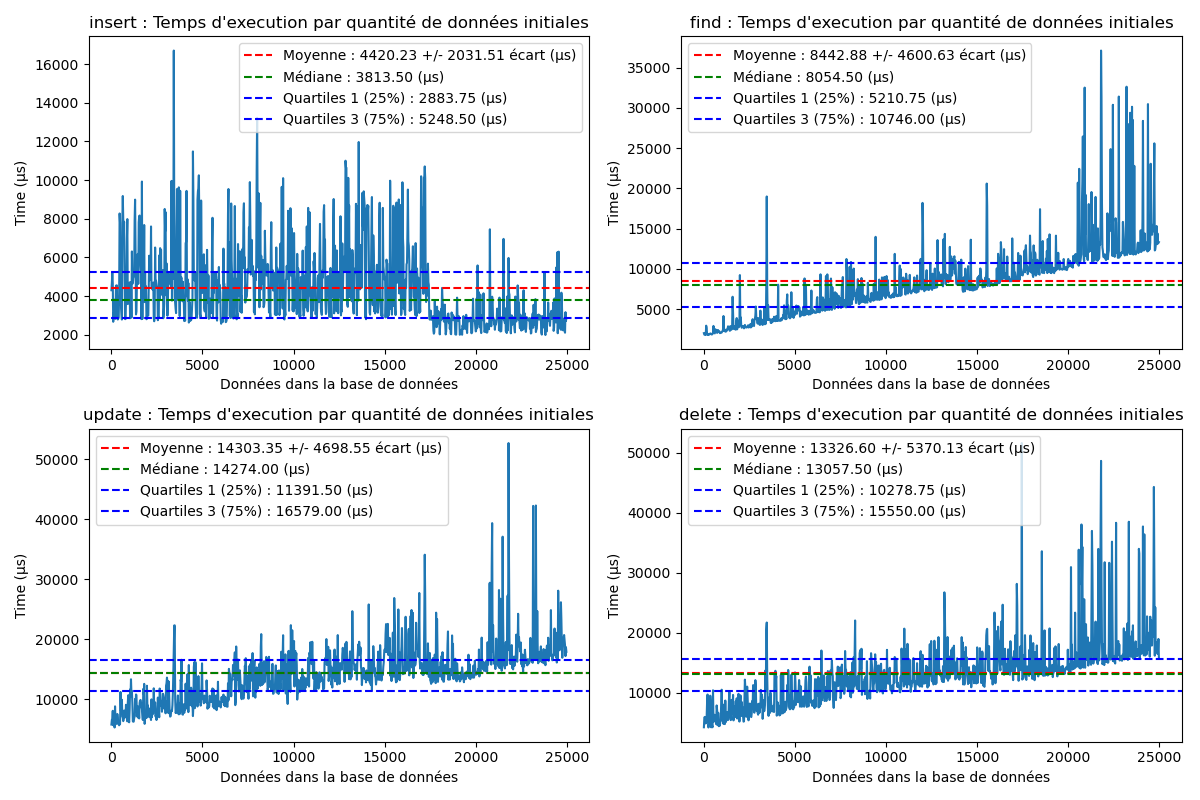
\includegraphics[width=0.8\textwidth]{../plots/MongoDB/replica_set/test_many_various_data.png}
            \caption{Performances des opérations CRUD multiples selon la quantitée de données dans la base.}
            \label{fig:mongo_replica_many_various}
        \end{figure}

        \subsection{Indexation}
        
            \subsubsection{Performances des Opérations uniques}

                \begin{figure}[H]
                    \centering
                    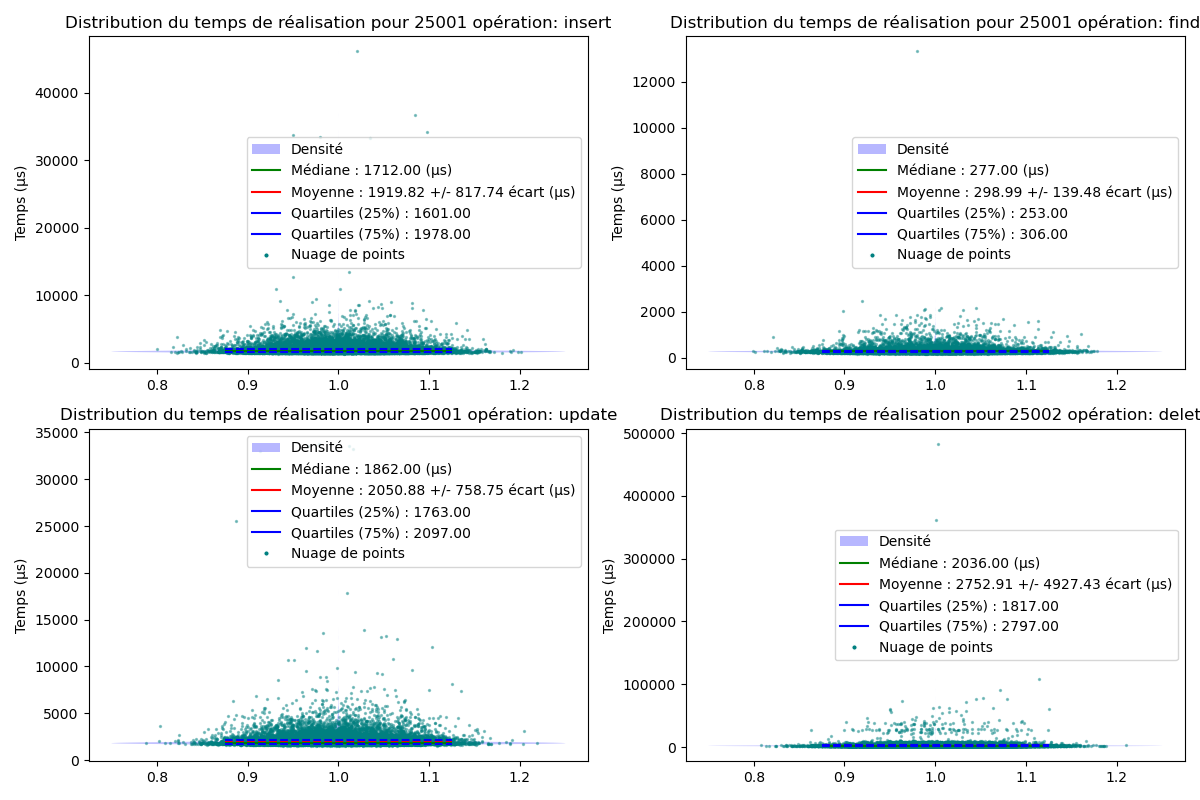
\includegraphics[width=0.8\textwidth]{../plots/MongoDB/replica_set_indexed/global_test_one.png}
                    \caption{Distribution des performances des opérations CRUD uniques.}
                    \label{fig:mongo_replica_global_one_indexed}
                \end{figure}

                \begin{figure}[H]
                    \centering
                    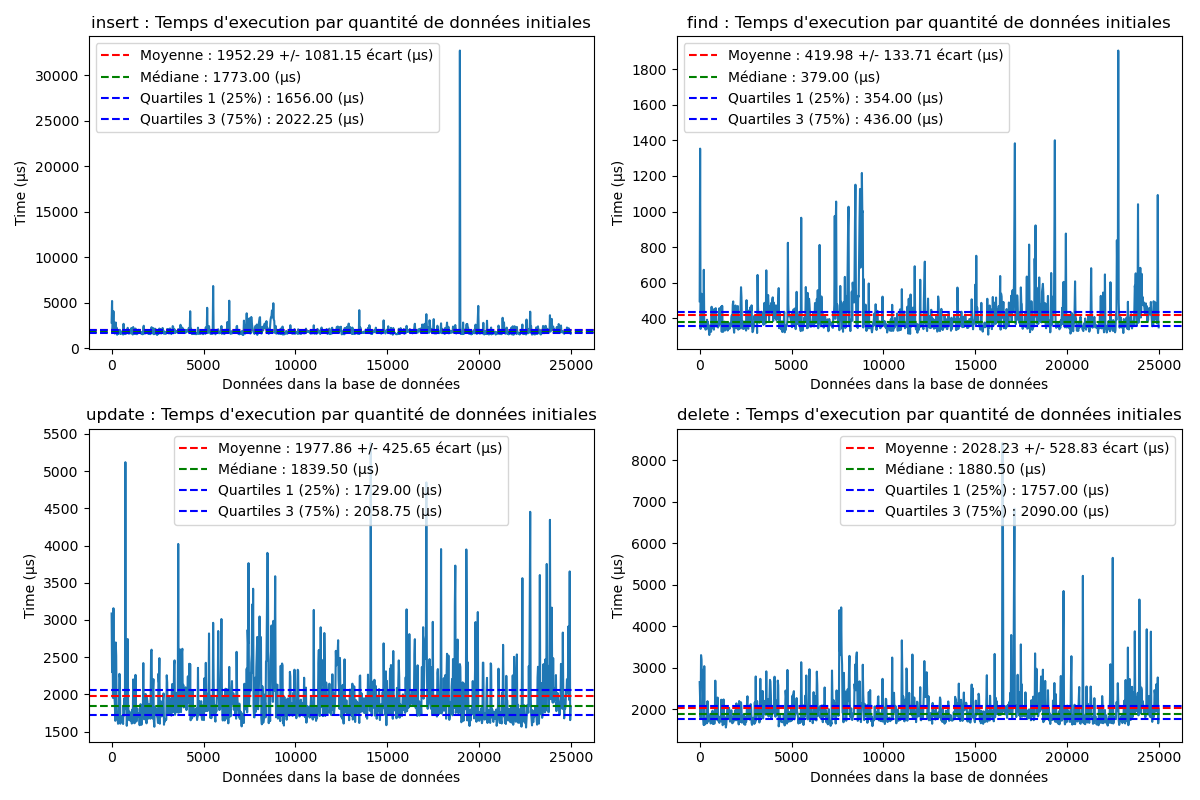
\includegraphics[width=0.8\textwidth]{../plots/MongoDB/replica_set_indexed/test_one_various_data.png}
                    \caption{Performances des opérations CRUD uniques selon la quantitée de données dans la base.}
                    \label{fig:mongo_replica_one_various_indexed}
                \end{figure}

            \subsubsection{Performances des Opérations avec données multiples}
                
                \begin{figure}[H]
                    \centering
                    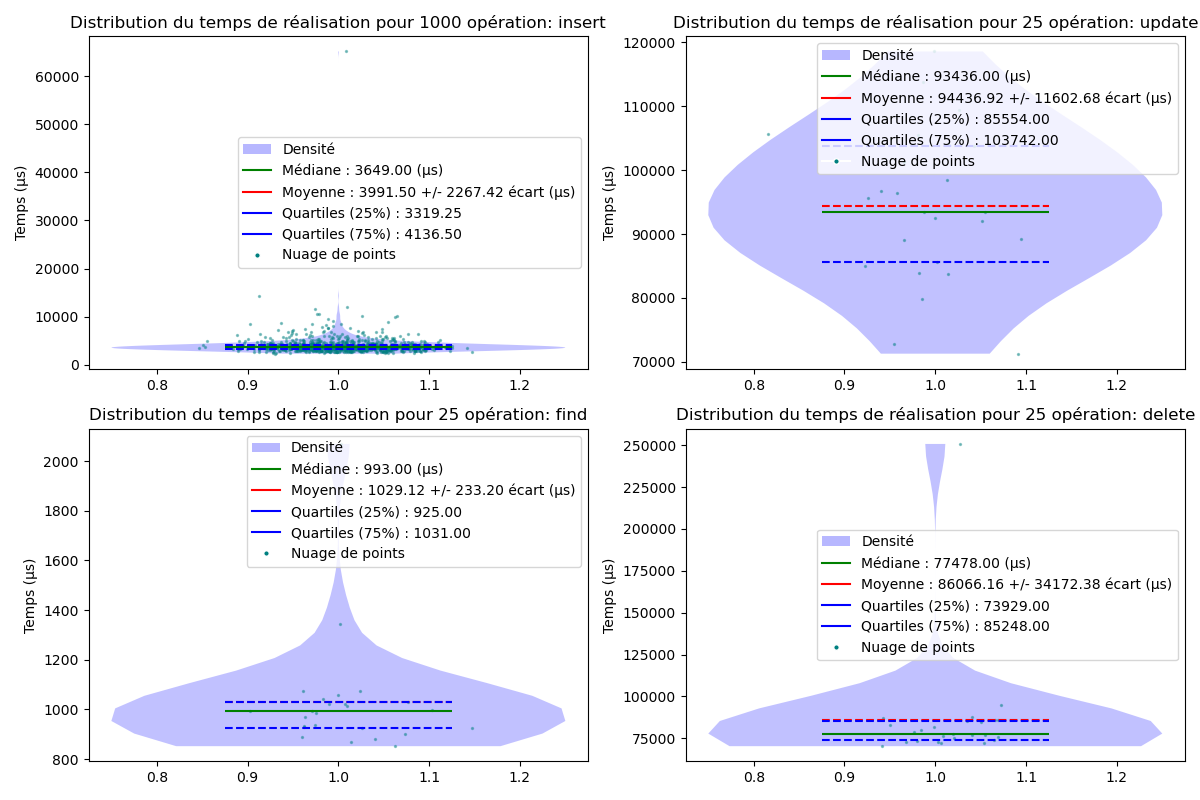
\includegraphics[width=0.8\textwidth]{../plots/MongoDB/replica_set_indexed/global_test_many.png}
                    \caption{Distribution des performances des opérations CRUD multiples.}
                    \label{fig:mongo_replica_global_many_indexed}
                \end{figure}

                \begin{figure}[H]
                    \centering
                    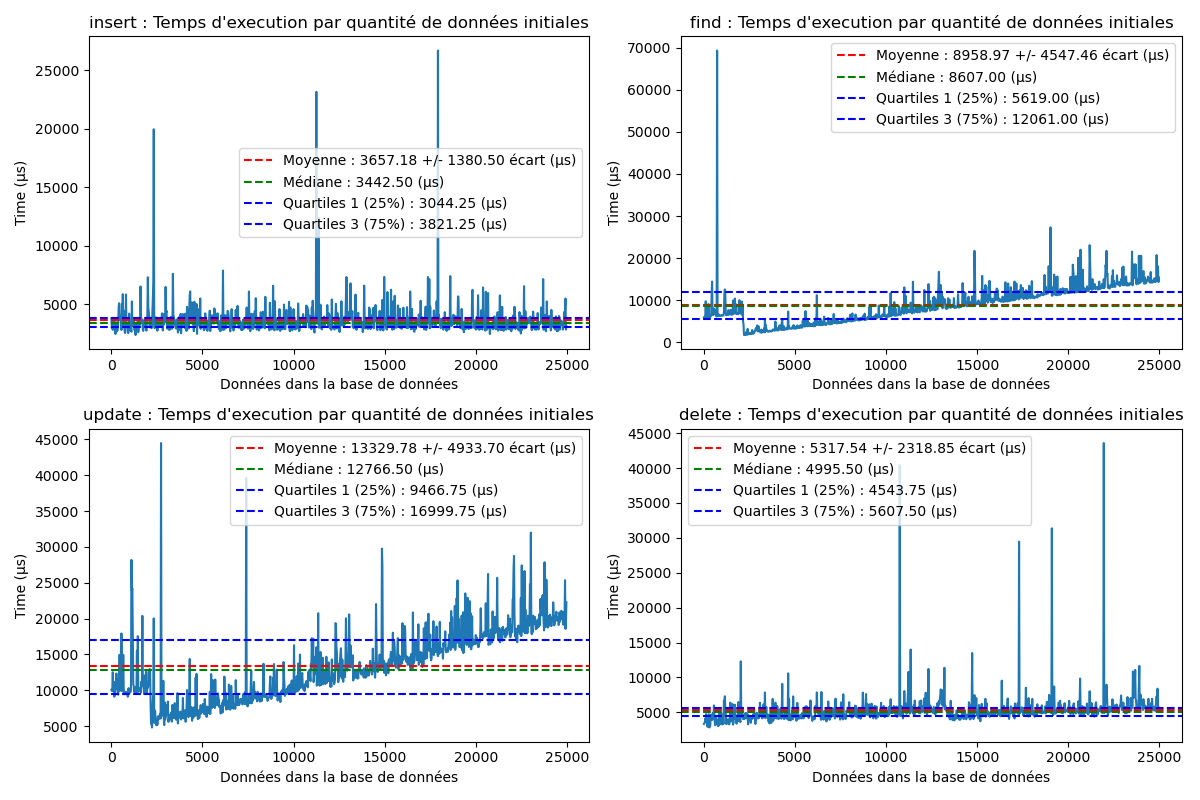
\includegraphics[width=0.8\textwidth]{../plots/MongoDB/replica_set_indexed/test_many_various_data.png}
                    \caption{Performances des opérations CRUD multiples selon la quantitée de données dans la base.}
                    \label{fig:mongo_replica_many_various_indexed}
                \end{figure}

        \subsection{Observations Globales sur la Réplication}
            \begin{card}
                Les résultats montrent que la réplication a un impact sur les performances des opérations CRUD. \\
                Les opérations de lecture et de mise à jour sont plus lentes en moyenne, tandis que l'insertion et la suppression sont plus rapides. \\
                Cela est dû au fait que les opérations de lecture et de mise à jour doivent être confirmées par plusieurs nœuds, ce qui augmente la latence. \\
                En revanche, l'insertion et la suppression peuvent être effectuées sur un seul nœud, ce qui réduit la latence. \\
                L'indexation améliore les performances des opérations de lecture et de mise à jour, mais a un impact négligeable sur l'insertion et la suppression. \\
                Les opérations multiples sont plus lentes que les opérations uniques, mais restent plus efficaces pour traiter de grandes quantités de données. \\
                Enfin, les performances des opérations CRUD sont plus stables avec l'indexation, ce qui réduit la variance des temps d'exécution. \\
            \end{card}


\section{Sharding}
    
    \subsection{Performances des Opérations uniques}

        \begin{figure}[H]
            \centering
            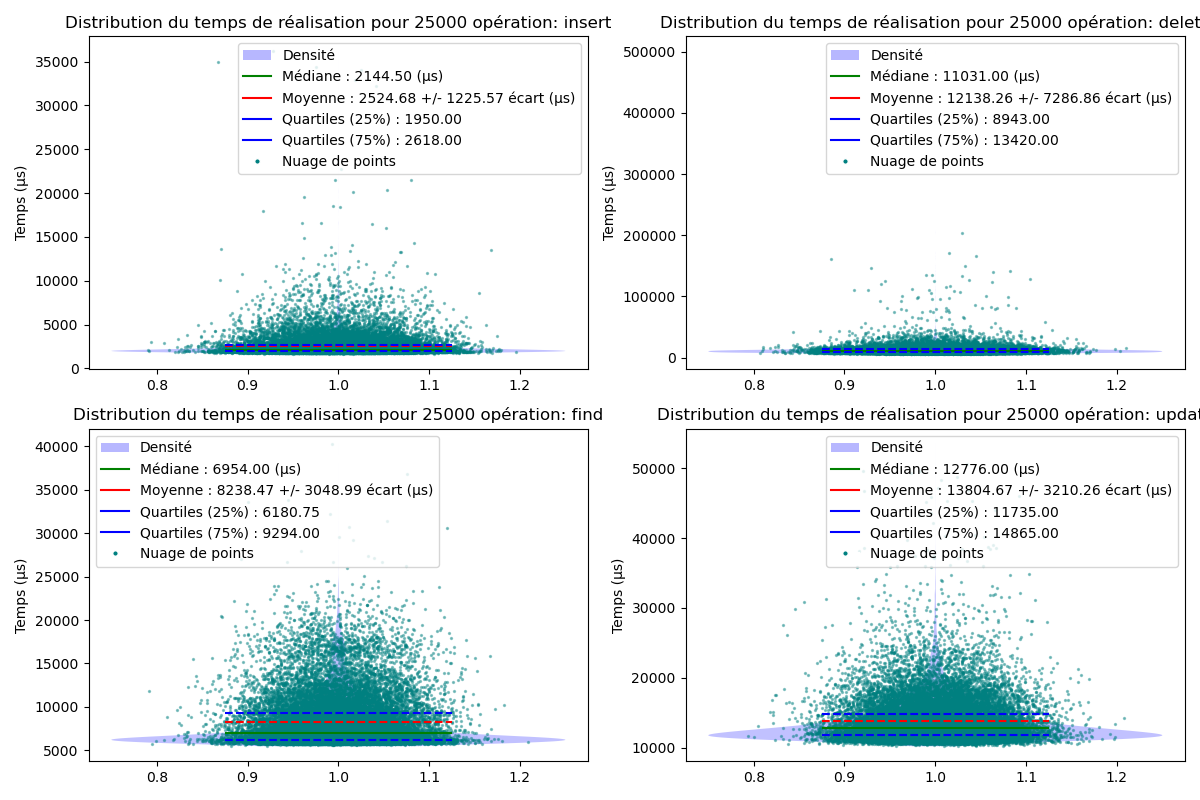
\includegraphics[width=0.8\textwidth]{../plots/MongoDB/sharding/global_test_one.png}
            \caption{Distribution des performances des opérations CRUD uniques.}
            \label{fig:mongo_sharded_global_one}
        \end{figure}

        \begin{figure}[H]
            \centering
            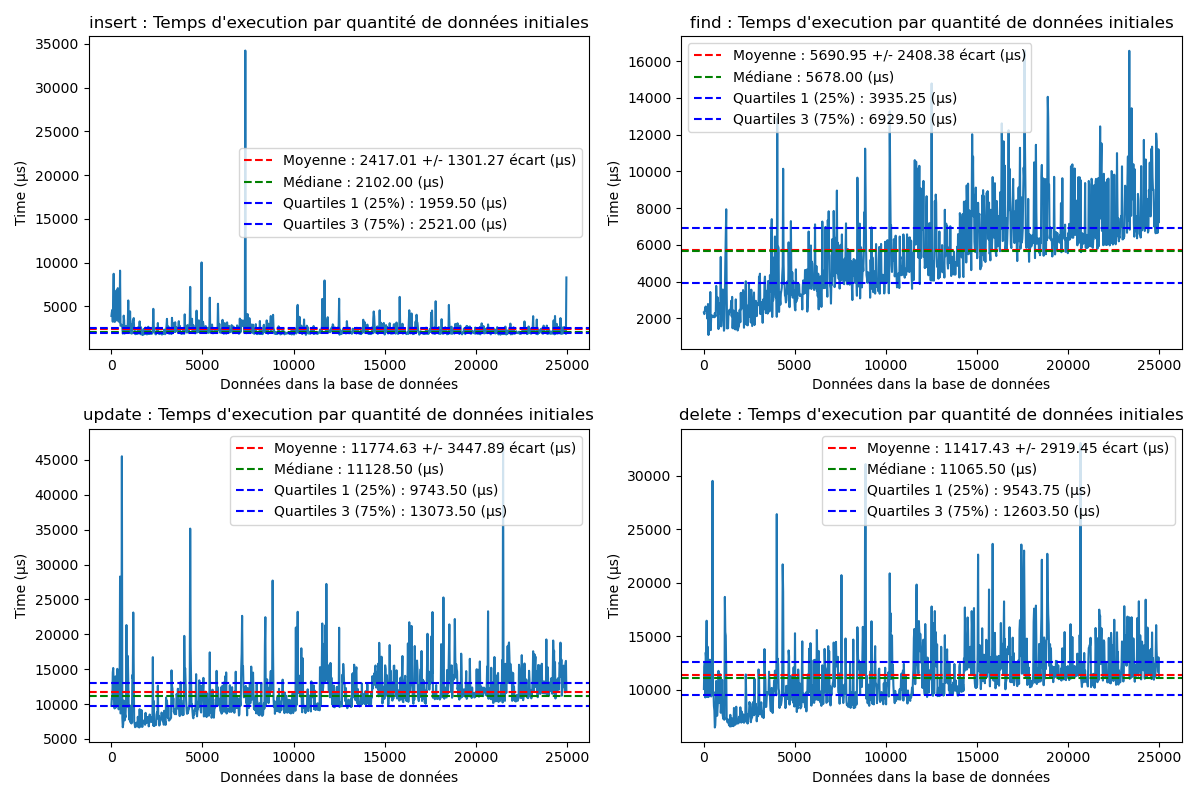
\includegraphics[width=0.8\textwidth]{../plots/MongoDB/sharding/test_one_various_data.png}
            \caption{Performances des opérations CRUD uniques selon la quantitée de données dans la base.}
            \label{fig:mongo_sharded_one_various}
        \end{figure}

    \subsection{Performances des Opérations avec données multiples}

        \begin{figure}[H]
            \centering
            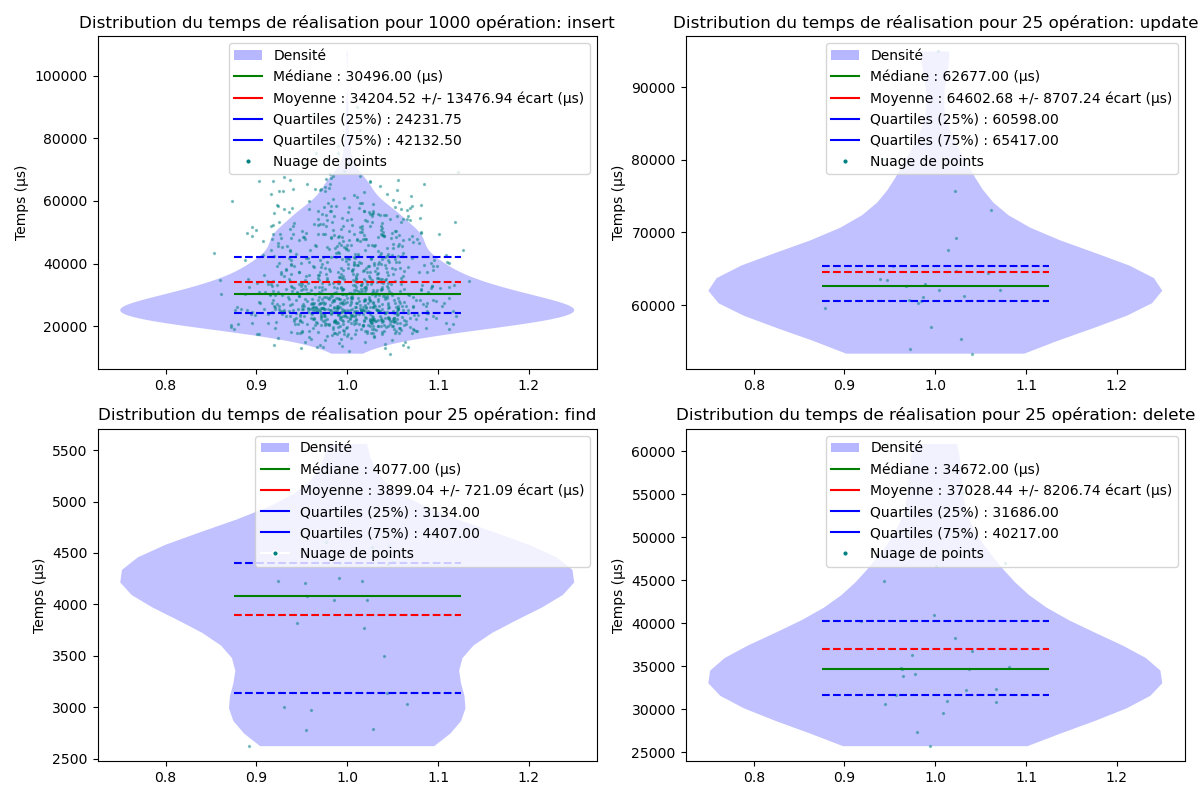
\includegraphics[width=0.8\textwidth]{../plots/MongoDB/sharding/global_test_many.png}
            \caption{Distribution des performances des opérations CRUD multiples.}
            \label{fig:mongo_sharded_global_many}
        \end{figure}

        \begin{figure}[H]
            \centering
            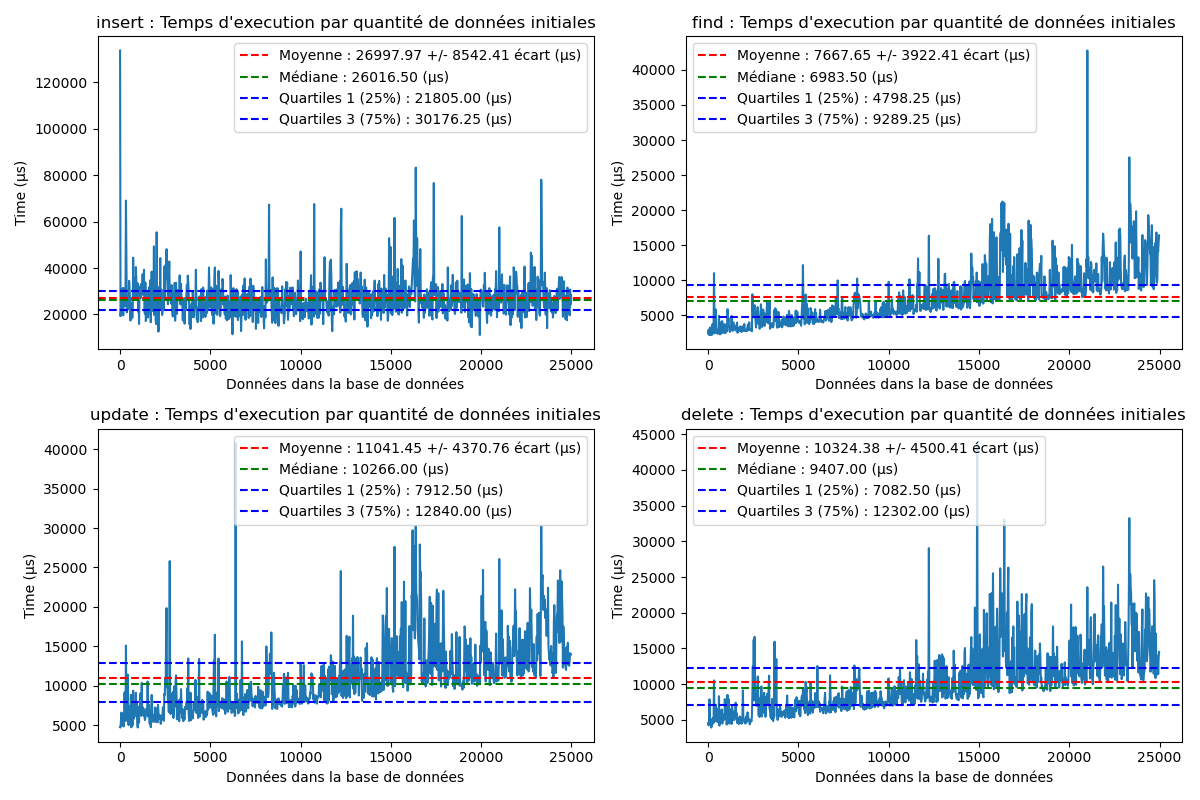
\includegraphics[width=0.8\textwidth]{../plots/MongoDB/sharding/test_many_various_data.png}
            \caption{Performances des opérations CRUD multiples selon la quantitée de données dans la base.}
            \label{fig:mongo_sharded_many_various}
        \end{figure}

        \subsection{Indexation}
        
            \subsubsection{Performances des Opérations uniques}

                \begin{figure}[H]
                    \centering
                    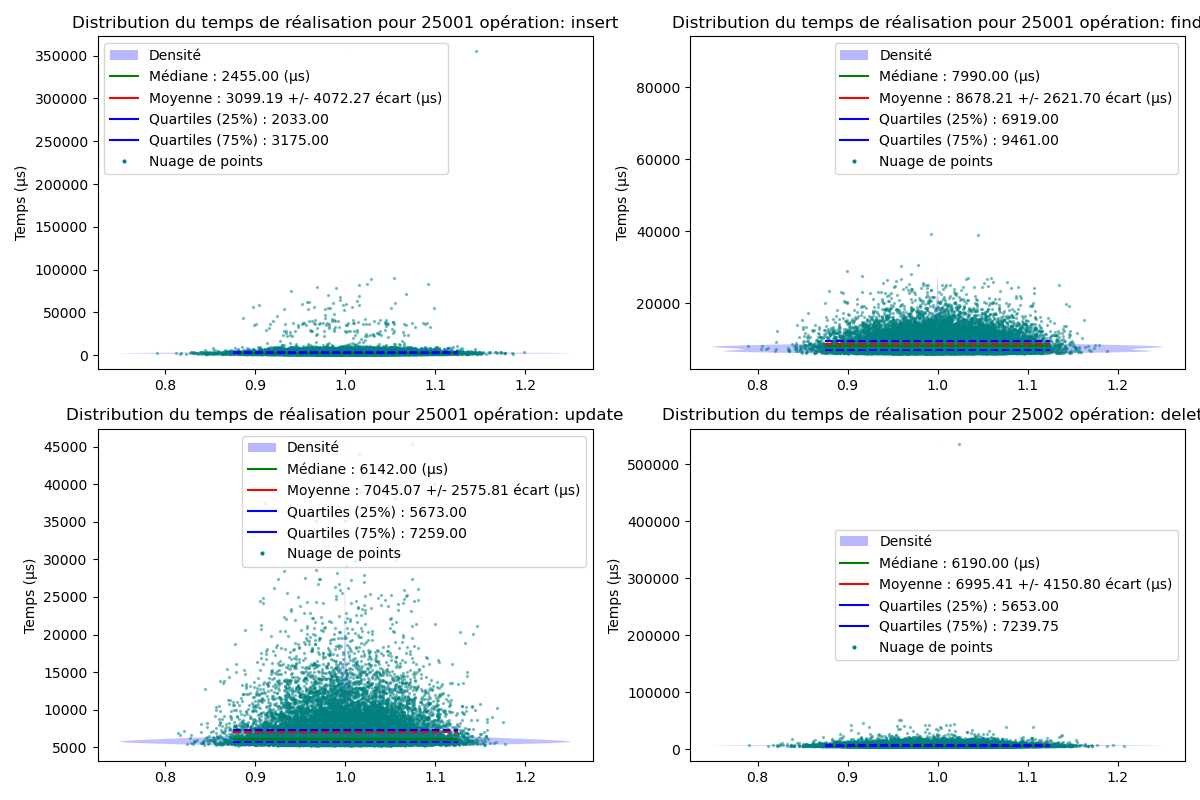
\includegraphics[width=0.8\textwidth]{../plots/MongoDB/sharding_indexed/global_test_one.png}
                    \caption{Distribution des performances des opérations CRUD uniques.}
                    \label{fig:mongo_sharded_global_one_indexed}
                \end{figure}

                \begin{figure}[H]
                    \centering
                    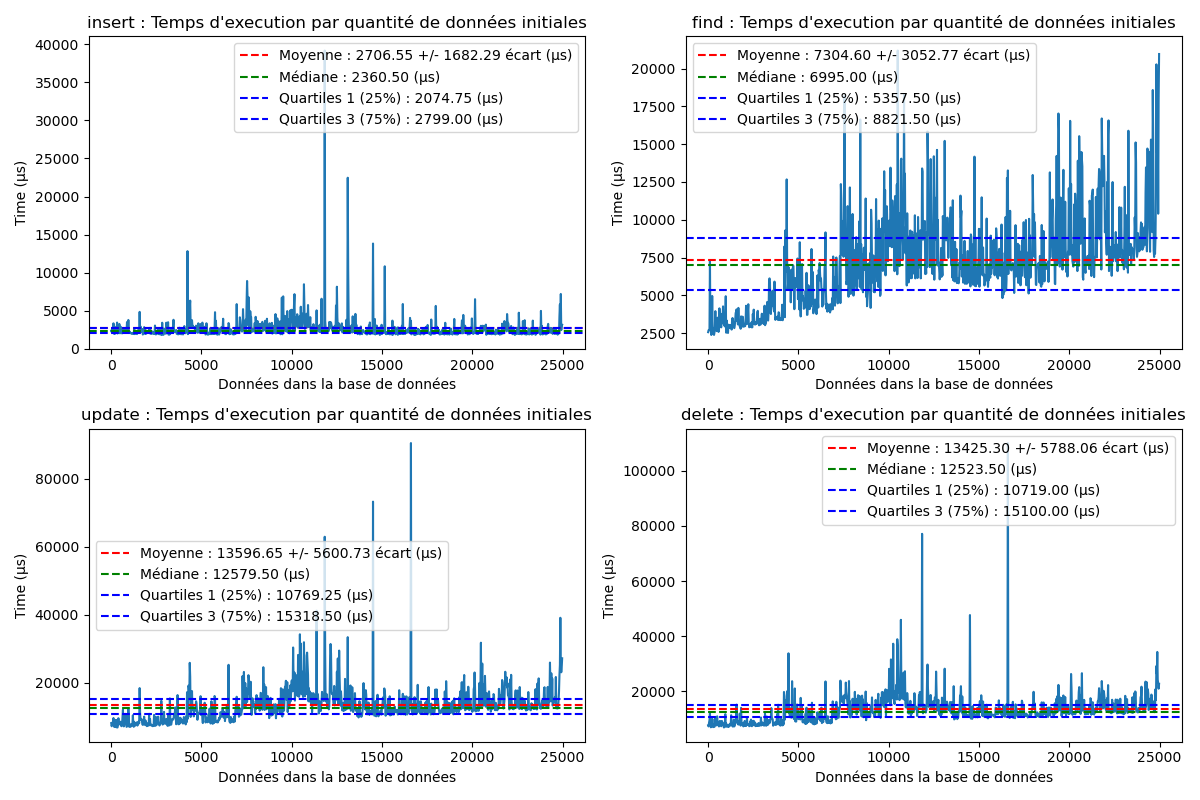
\includegraphics[width=0.8\textwidth]{../plots/MongoDB/sharding_indexed/test_one_various_data.png}
                    \caption{Performances des opérations CRUD uniques selon la quantitée de données dans la base.}
                    \label{fig:mongo_sharded_one_various_indexed}
                \end{figure}
            
            \subsubsection{Performances des Opérations avec données multiples}
                
                \begin{figure}[H]
                    \centering
                    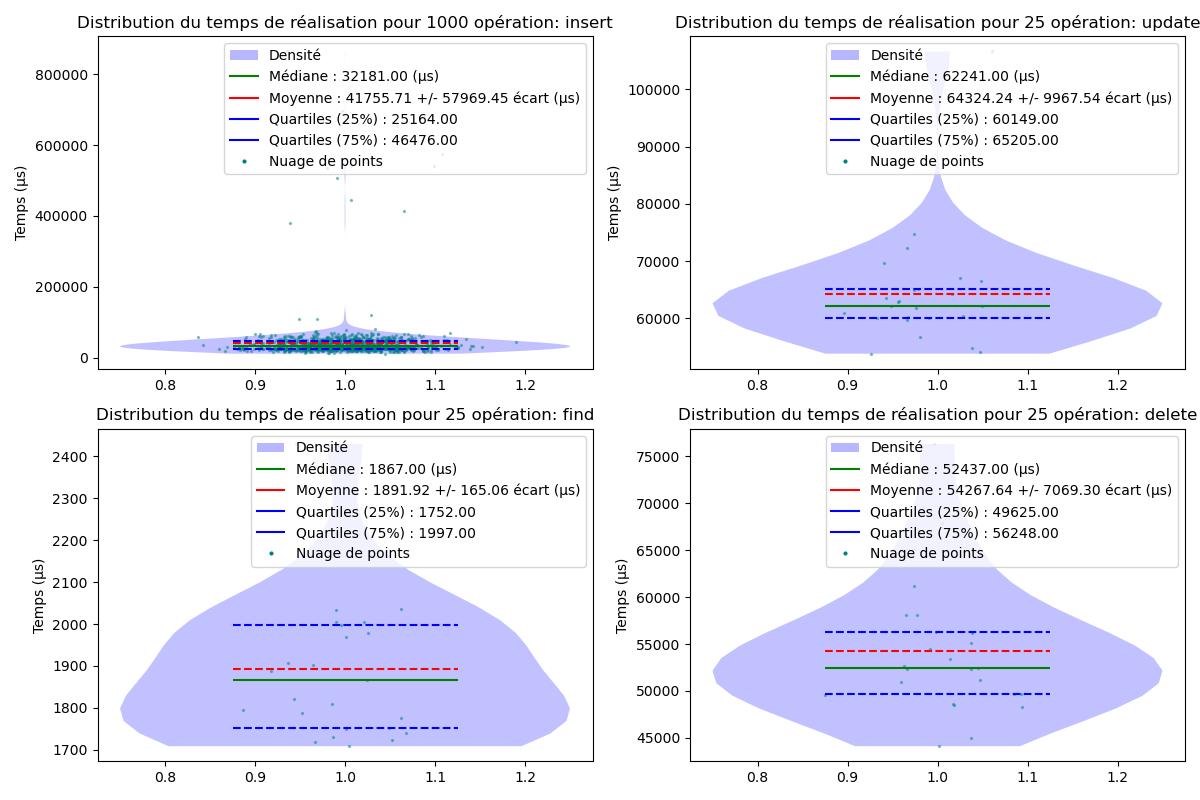
\includegraphics[width=0.8\textwidth]{../plots/MongoDB/sharding_indexed/global_test_many.png}
                    \caption{Distribution des performances des opérations CRUD multiples.}
                    \label{fig:mongo_sharded_global_many_indexed}
                \end{figure}

                \begin{figure}[H]
                    \centering
                    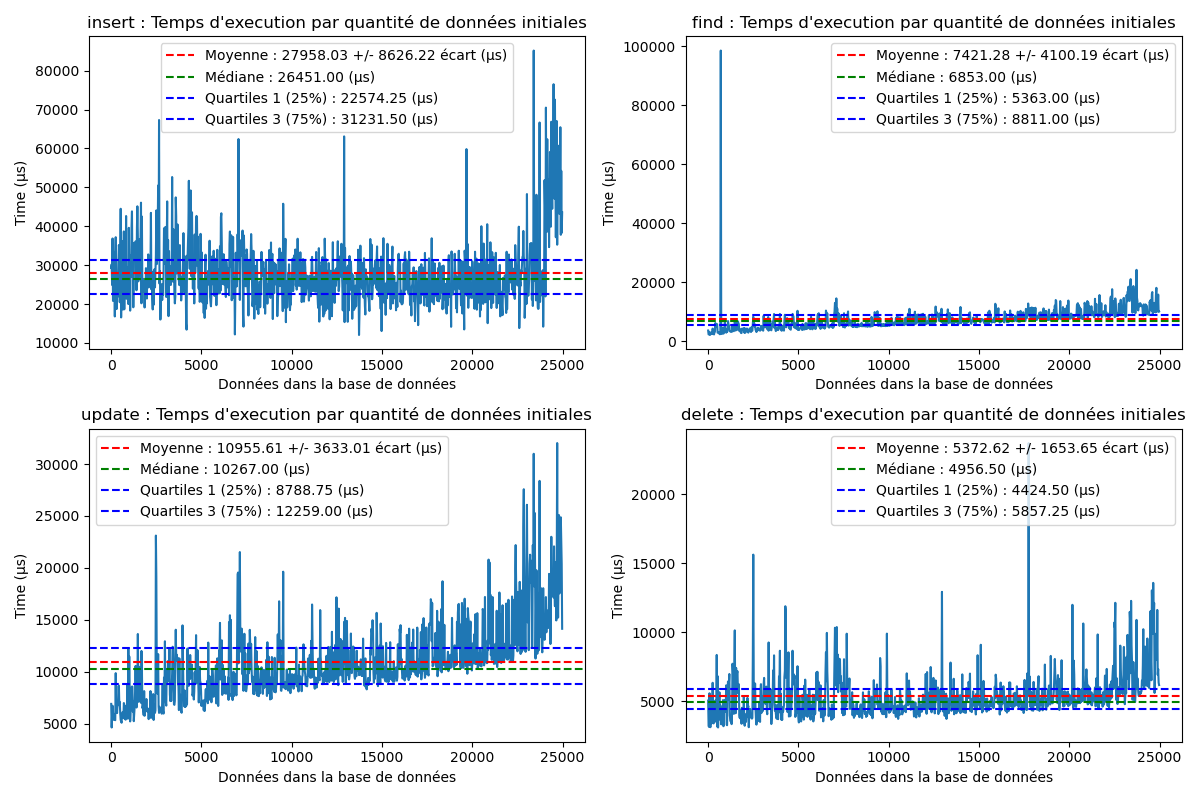
\includegraphics[width=0.8\textwidth]{../plots/MongoDB/sharding_indexed/test_many_various_data.png}
                    \caption{Performances des opérations CRUD multiples selon la quantitée de données dans la base.}
                    \label{fig:mongo_sharded_many_various_indexed}
                \end{figure}


        \subsection{Observations Globales sur la fragmentation}
            \begin{card}
                Les résultats montrent que la fragmentation améliore les performances des opérations CRUD pa rapport à la réplication. \\
                Les opérations sont plus rapides ou quasiment aussi performantes et surtout plus stables.
                Cela est dû au fait que les opérations de lecture et de mise à jour peuvent être parallélisées sur plusieurs nœuds, tandis que l'insertion et la suppression nécessitent une coordination entre les nœuds. \\
                Entre la version indexée et non indexée, on n'observe pas d'amélioration significative des performances. \\
                Cela peut être du au fait que le shard se fait déjà sur un champ indexé (id) et que les opérations sont déjà optimisées et les index peu utiles, voir même contre-productifs. \\
                Il faudrait certainement avoir des operations plus adaptées et un schéma d'indexation plus optimisée pour voir apparâitre des différences significatives. \\
                De plus, comparativement au mode standalone, les performances sont moindre contrairement aux attentes. \\
                Cela peut être dû au fait que la configuration n'est pas optimisée, que les requêtes sont envoyées au noeud le plus proche et non au noeud primaires ce qui engendre des coûts de latence supplémentaires. \\
                Néanmoins, le sharding reste intéressant, avec un configuration optimisée, pour des applications nécessitant une haute disponibilité et une distribution des données. \\
            \end{card}
                

\chapter{Résultats et Analyses pour MySQL}

\section{MySQL Standalone}

    \subsection{Performances des Opérations uniques}

        \begin{figure}[H]
            \centering
            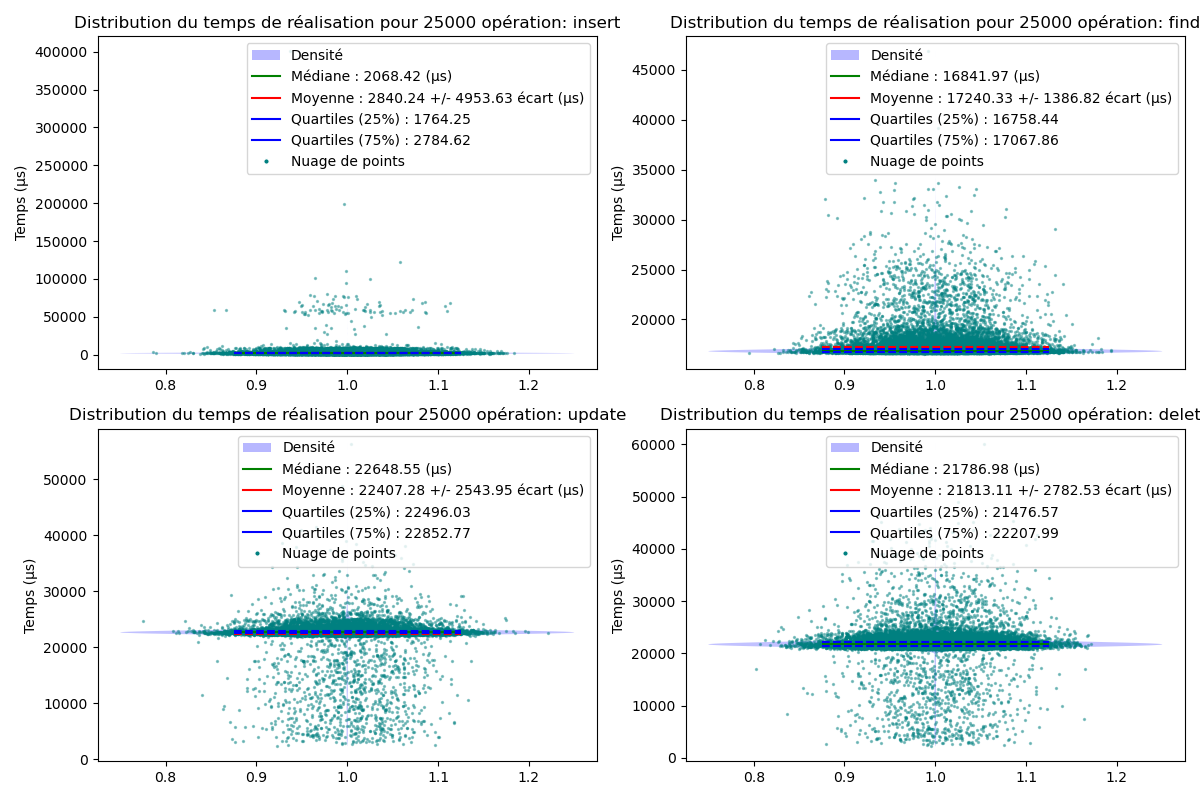
\includegraphics[width=0.8\textwidth]{../plots/MySQL/standalone/global_test_one.png}
            \caption{Distribution des performances des opérations CRUD uniques.}
            \label{fig:mysql_standalone_global_one}
        \end{figure}

        \begin{figure}[H]
            \centering
            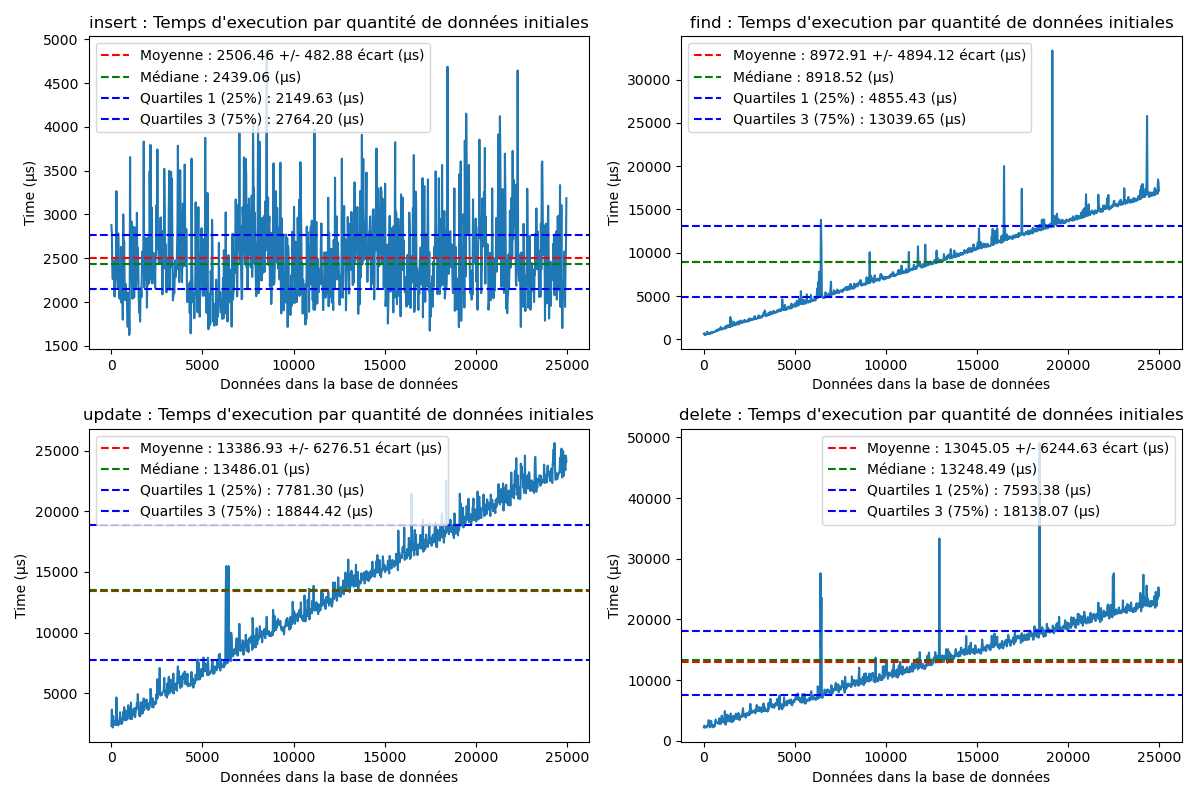
\includegraphics[width=0.8\textwidth]{../plots/MySQL/standalone/test_one_various_data.png}
            \caption{Performances des opérations CRUD uniques selon la quantitée de données dans la base.}
            \label{fig:mysql_standalone_one_various}
        \end{figure}

    \subsection{Performances des Opérations avec données multiples}

        \begin{figure}[H]
            \centering
            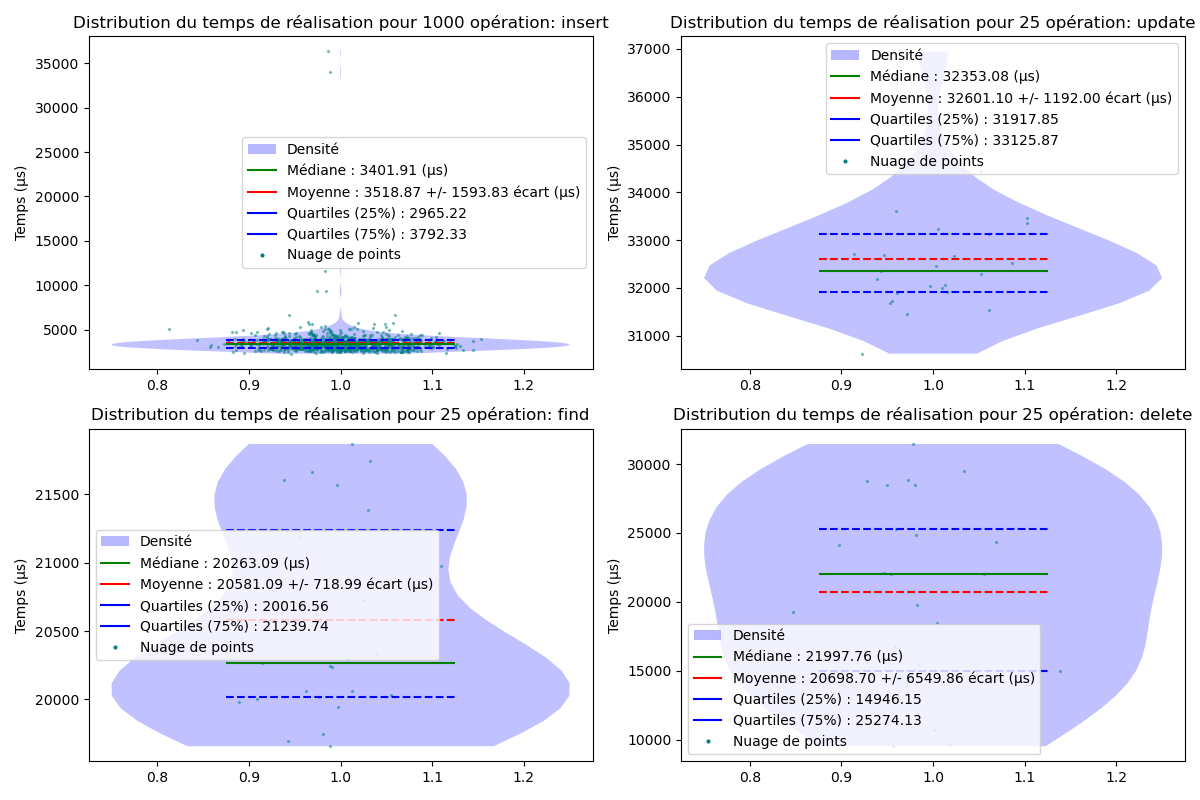
\includegraphics[width=0.8\textwidth]{../plots/MySQL/standalone/global_test_many.png}
            \caption{Distribution des performances des opérations CRUD multiples.}
            \label{fig:mysql_standalone_global_many}
        \end{figure}

        \begin{figure}[H]
            \centering
            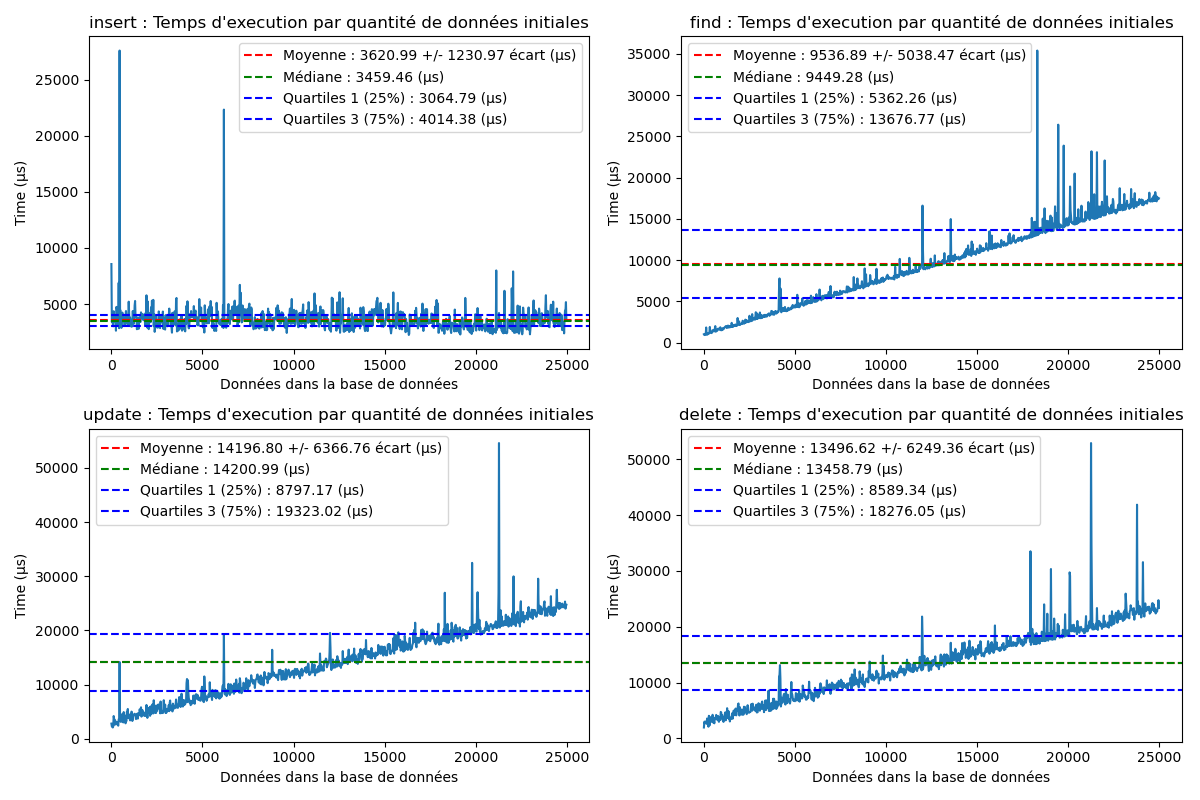
\includegraphics[width=0.8\textwidth]{../plots/MySQL/standalone/test_many_various_data.png}
            \caption{Performances des opérations CRUD multiples selon la quantitée de données dans la base.}
            \label{fig:mysql_standalone_many_various}
        \end{figure}

        \subsection{Indexation}
        
            \subsubsection{Performances des Opérations uniques}

                \begin{figure}[H]
                    \centering
                    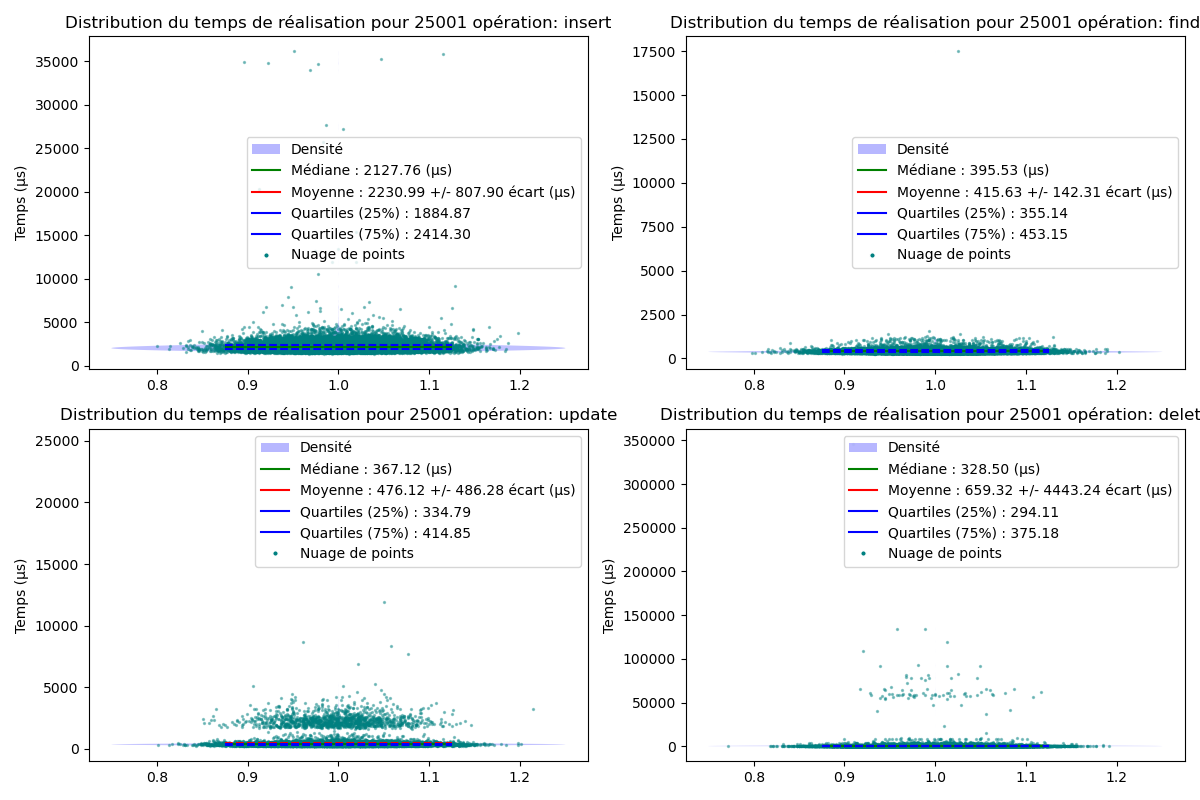
\includegraphics[width=0.8\textwidth]{../plots/MySQL/standalone_indexed/global_test_one.png}
                    \caption{Distribution des performances des opérations CRUD uniques.}
                    \label{fig:mysql_standalone_global_one_indexed}
                \end{figure}

                \begin{figure}[H]
                    \centering
                    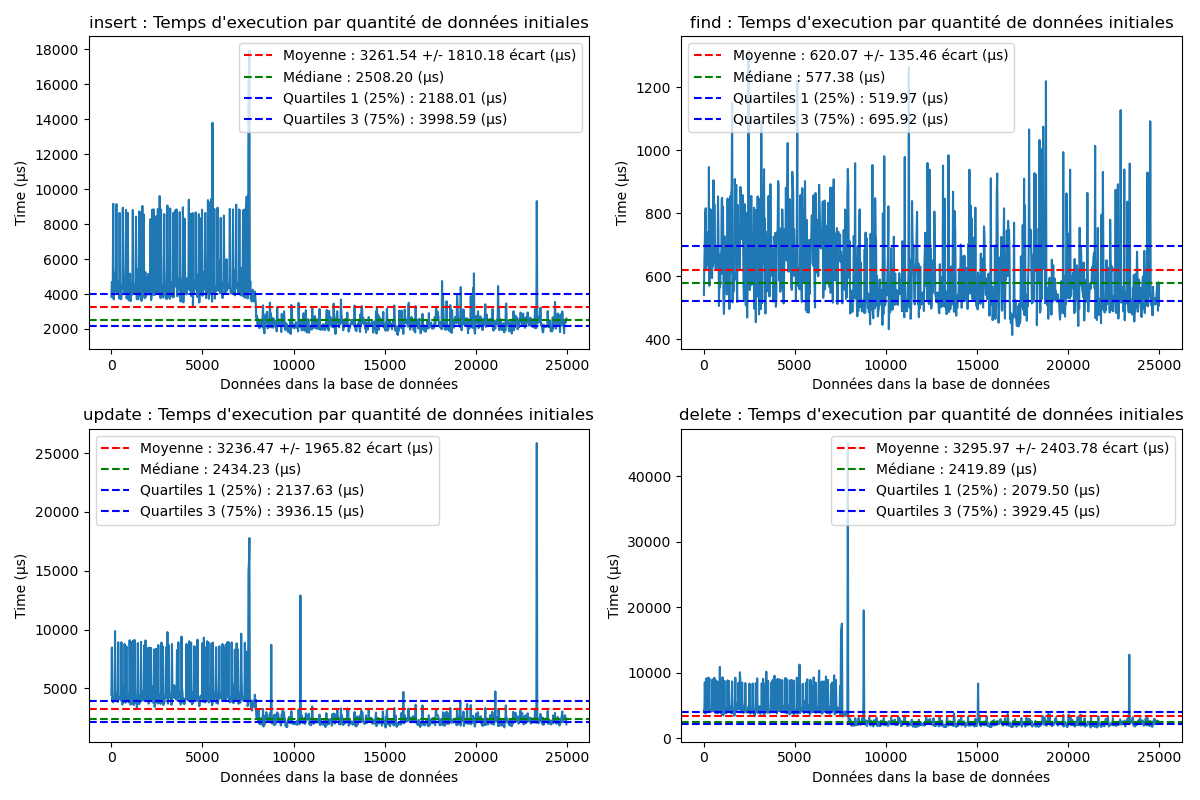
\includegraphics[width=0.8\textwidth]{../plots/MySQL/standalone_indexed/test_one_various_data.png}
                    \caption{Performances des opérations CRUD uniques selon la quantitée de données dans la base.}
                    \label{fig:mysql_standalone_global_one_various_indexed}
                \end{figure}

            \subsubsection{Performances des Opérations avec données multiples}  
                
                \begin{figure}[H]
                    \centering
                    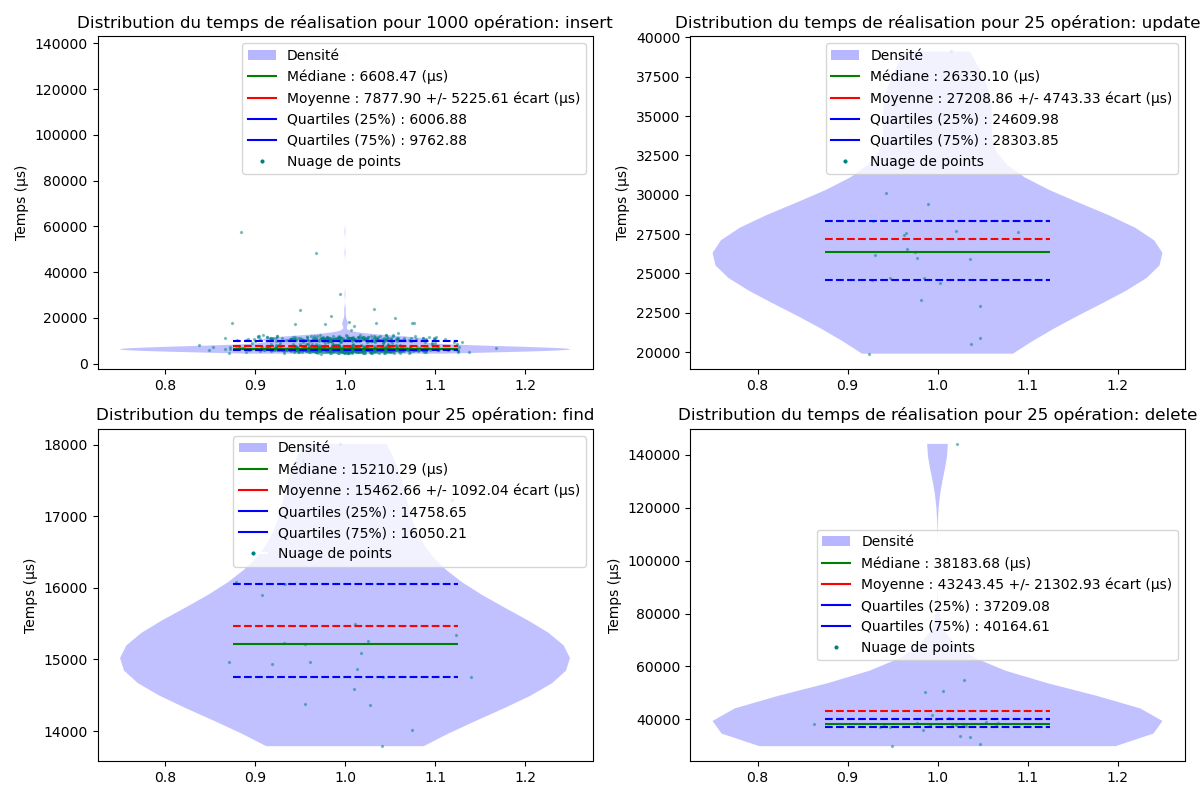
\includegraphics[width=0.8\textwidth]{../plots/MySQL/standalone_indexed/global_test_many.png}
                    \caption{Distribution des performances des opérations CRUD multiples.}
                    \label{fig:mysql_standalone_global_many_indexed}
                \end{figure}

                \begin{figure}[H]
                    \centering
                    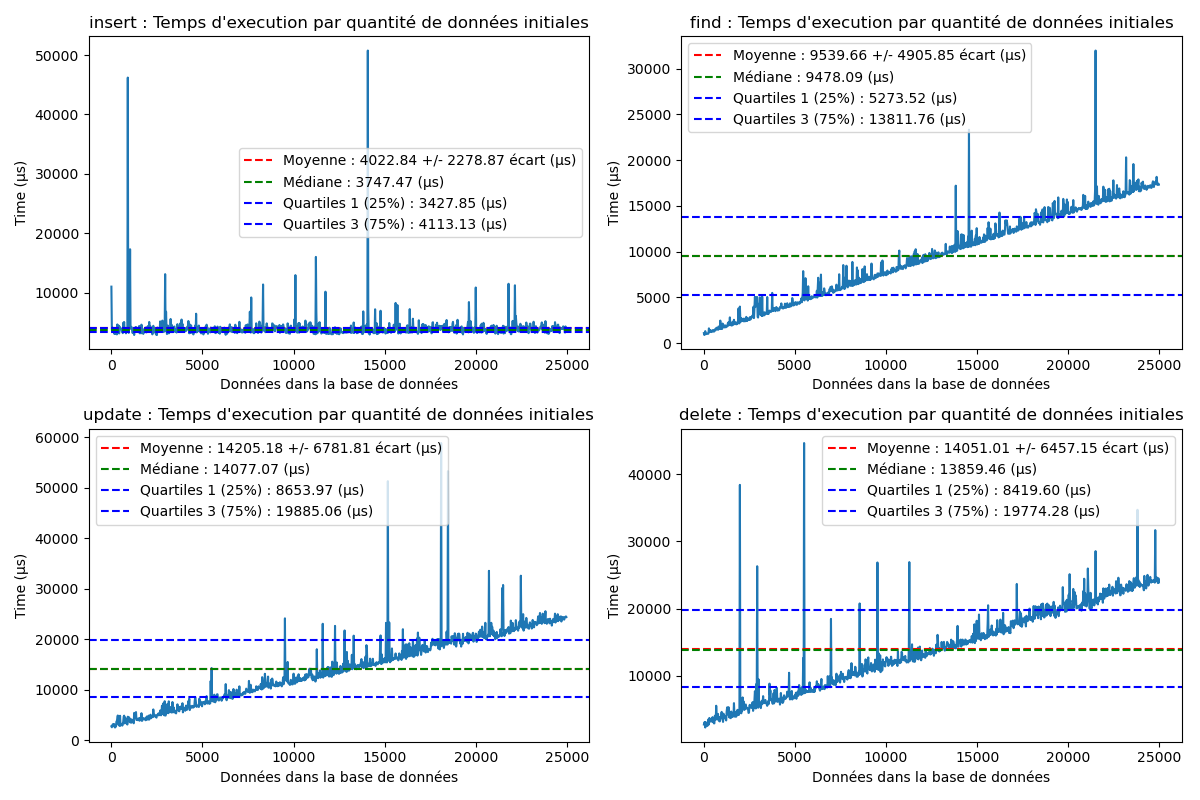
\includegraphics[width=0.8\textwidth]{../plots/MySQL/standalone_indexed/test_many_various_data.png}
                    \caption{Performances des opérations CRUD multiples selon la quantitée de données dans la base.}
                    \label{fig:mysql_standalone_global_many_various_indexed}
                \end{figure}

        \subsection{Observations Globales sur MySQL Standalone}

            \begin{card}
                Les résultats montrent que MySQL est moins performant sans indexation pour les opérations uniques que MongoDB. \\
                Les obeservations selon la quantité de données dans la base sont similaires à celles de MongoDB, avec néanmoins un coefficient plus important dans le cas de la modification.
                Avec indexation,on observe pour les opérations à l'exception de la recherche, une variance importante, avec un temps d'execution long, jusqu'à un certain point où les opérations deviennentconstantes en moyennes et avec des performances similaires à MongoDB. \\
                Néanmoins, des imprécisions peuvent être dues à la façon dont les temps d'execution sont mesurés.
            \end{card}

\section{MySQL Cluster}
            
    \subsection{Performances des Opérations uniques}

        \begin{figure}[H]
            \centering
            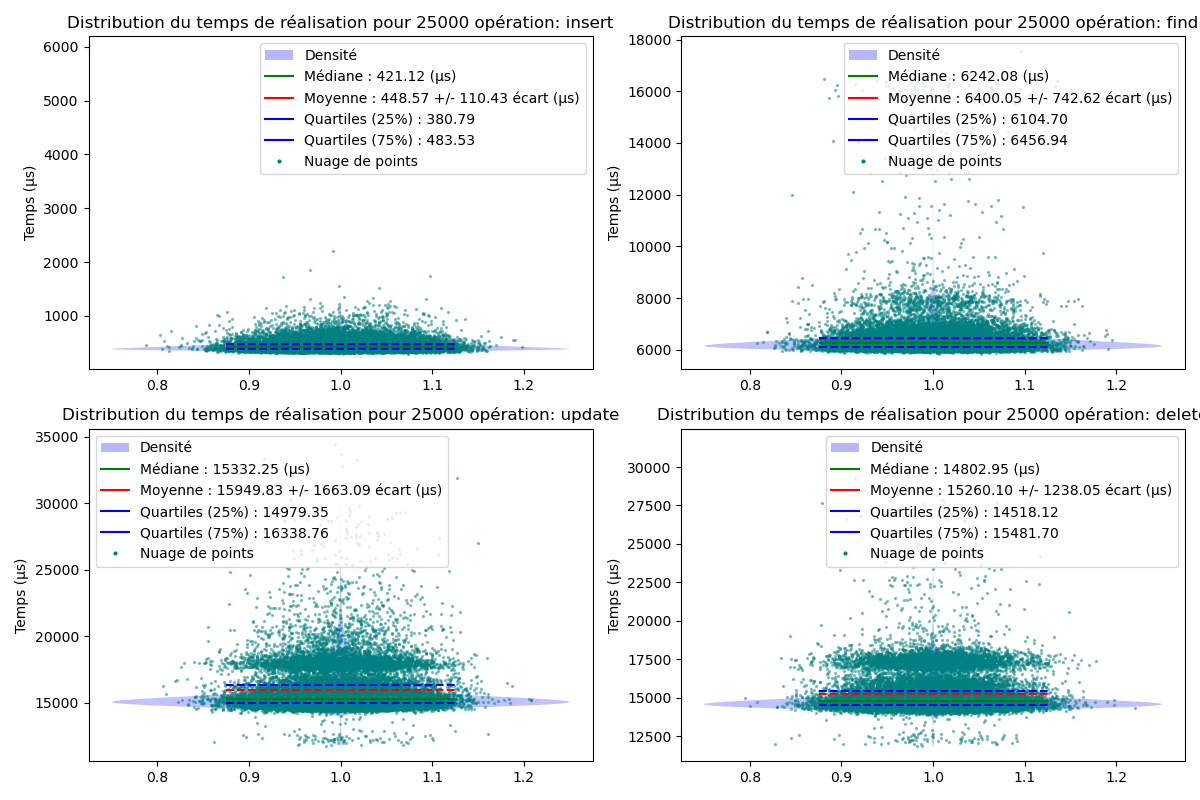
\includegraphics[width=0.8\textwidth]{../plots/MySQL/sharding/global_test_one.png}
            \caption{Distribution des performances des opérations CRUD uniques.}
            \label{fig:mysql_cluster_global_one}
        \end{figure}

        \begin{figure}[H]
            \centering
            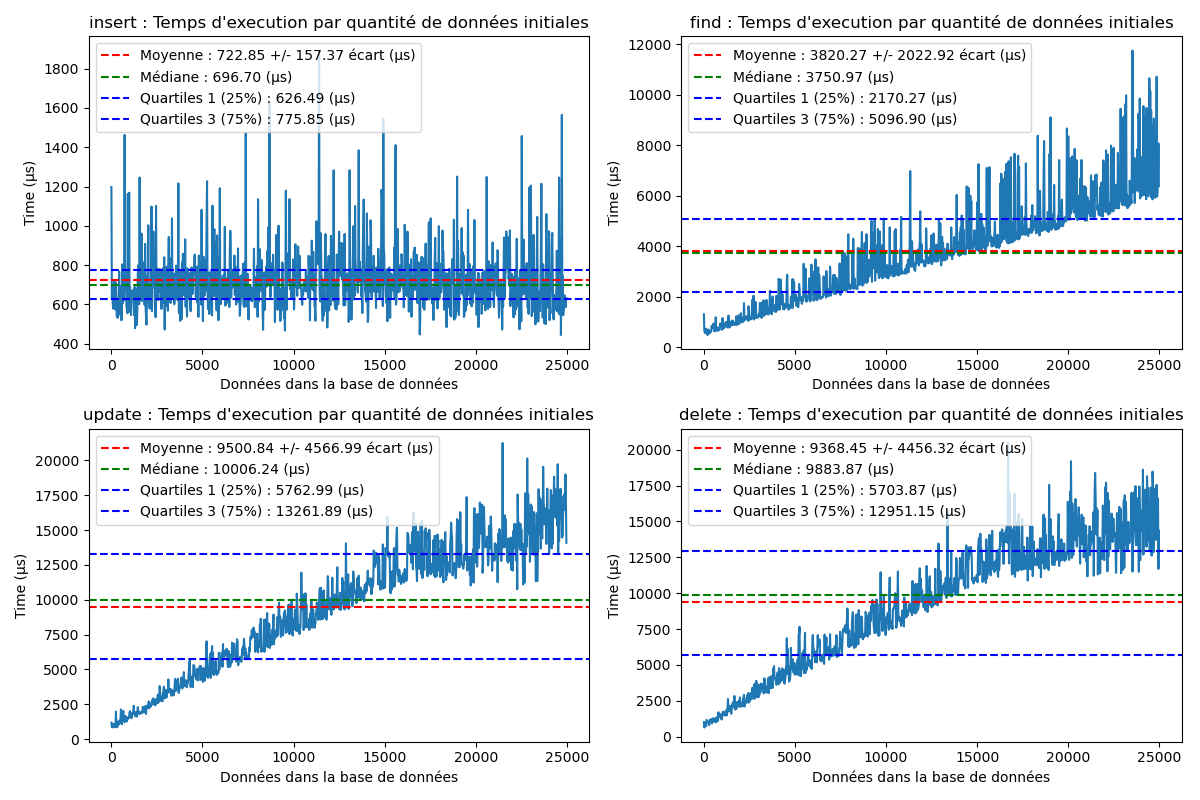
\includegraphics[width=0.8\textwidth]{../plots/MySQL/sharding/test_one_various_data.png}
            \caption{Performances des opérations CRUD uniques selon la quantitée de données dans la base.}
            \label{fig:mysql_cluster_one_various}
        \end{figure}

    \subsection{Performances des Opérations avec données multiples}

        \begin{figure}[H]
            \centering
            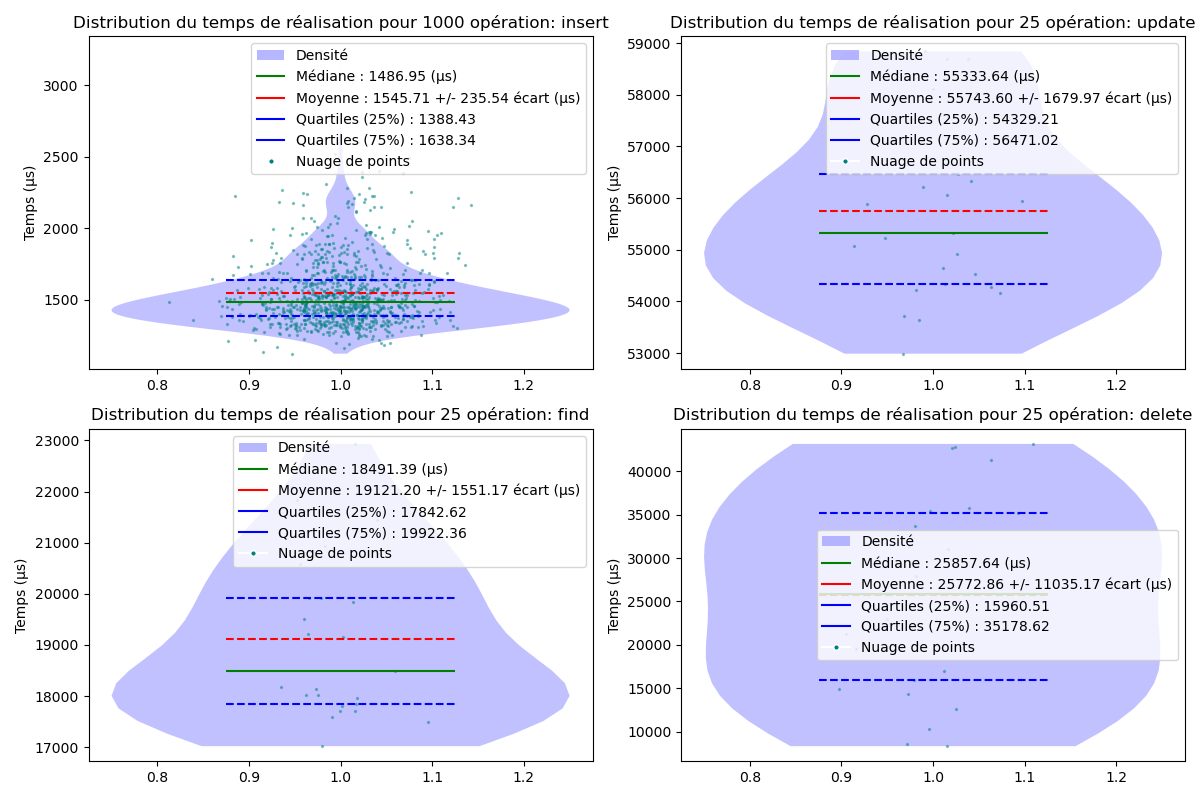
\includegraphics[width=0.8\textwidth]{../plots/MySQL/sharding/global_test_many.png}
            \caption{Distribution des performances des opérations CRUD multiples.}
            \label{fig:mysql_cluster_global_many}
        \end{figure}

        \begin{figure}[H]
            \centering
            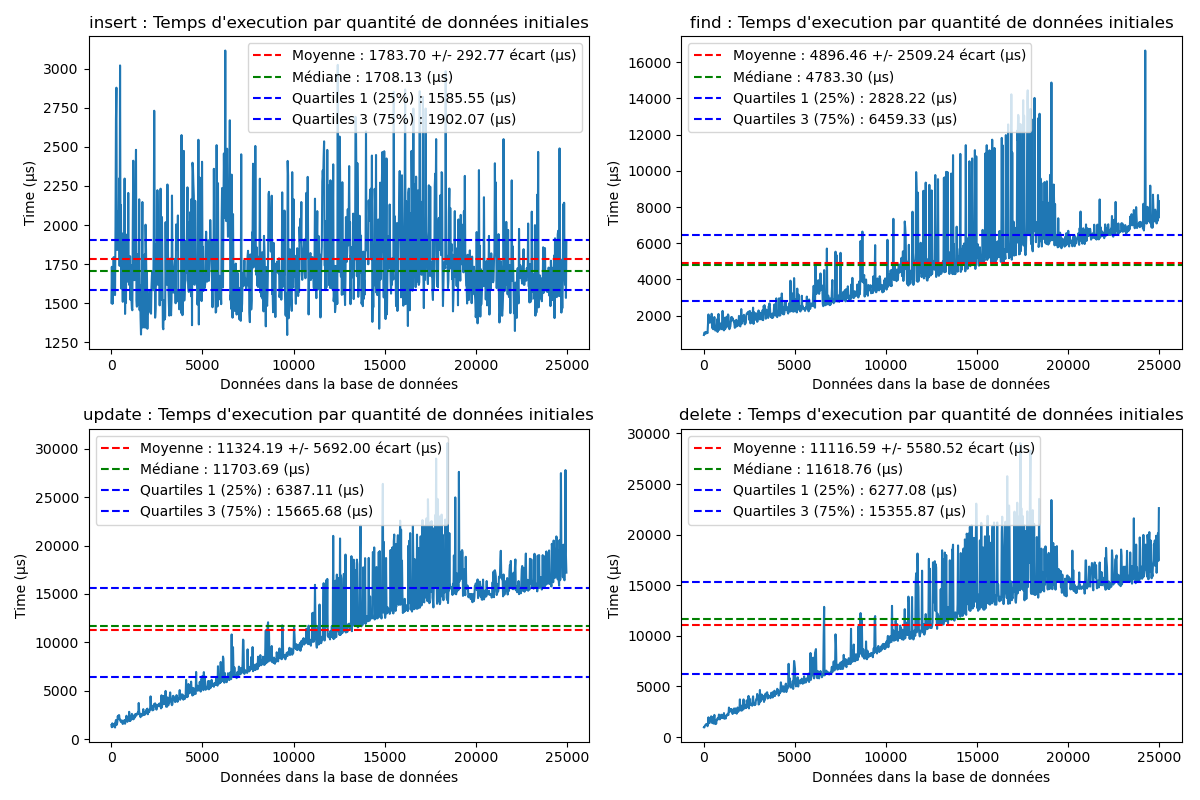
\includegraphics[width=0.8\textwidth]{../plots/MySQL/sharding/test_many_various_data.png}
            \caption{Performances des opérations CRUD multiples selon la quantitée de données dans la base.}
            \label{fig:mysql_cluster_many_various}
        \end{figure}

        \subsection{Indexation}
        
            \subsubsection{Performances des Opérations uniques}

                \begin{figure}[H]
                    \centering
                    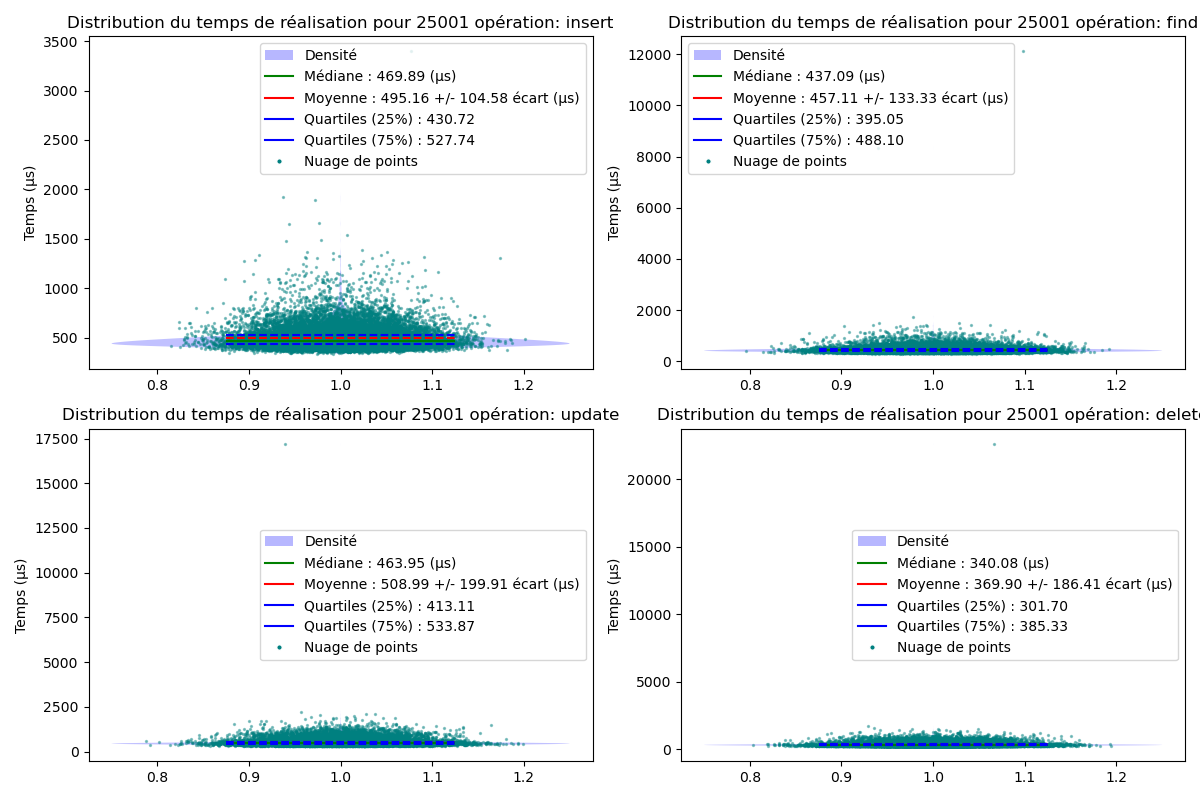
\includegraphics[width=0.8\textwidth]{../plots/MySQL/sharding_indexed/global_test_one.png}
                    \caption{Distribution des performances des opérations CRUD uniques.}
                    \label{fig:mysql_cluster_global_one_indexed}
                \end{figure}

                \begin{figure}[H]
                    \centering
                    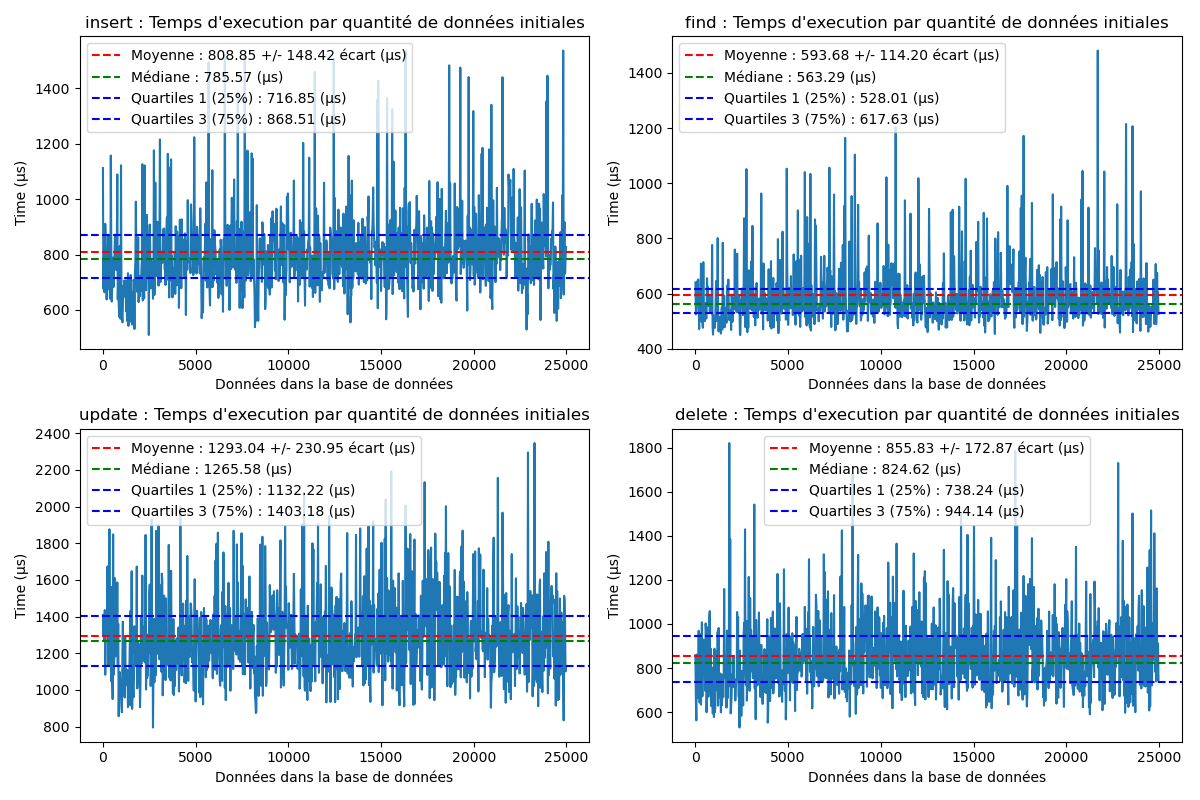
\includegraphics[width=0.8\textwidth]{../plots/MySQL/sharding_indexed/test_one_various_data.png}
                    \caption{Performances des opérations CRUD uniques selon la quantitée de données dans la base.}
                    \label{fig:mysql_cluster_global_one_various_indexed}
                \end{figure}

            \subsubsection{Performances des Opérations avec données multiples}
                
                \begin{figure}[H]
                    \centering
                    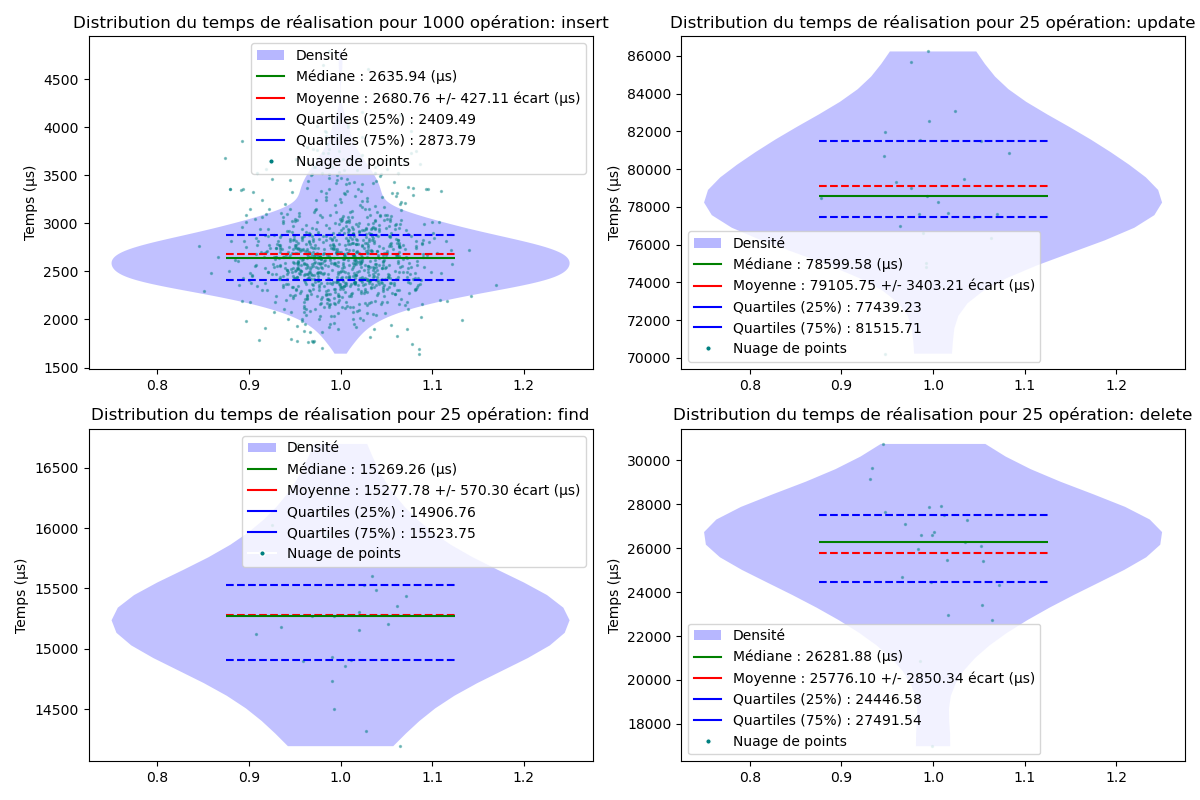
\includegraphics[width=0.8\textwidth]{../plots/MySQL/sharding_indexed/global_test_many.png}
                    \caption{Distribution des performances des opérations CRUD multiples.}
                    \label{fig:mysql_cluster_global_many_indexed}
                \end{figure}

                \begin{figure}[H]
                    \centering
                    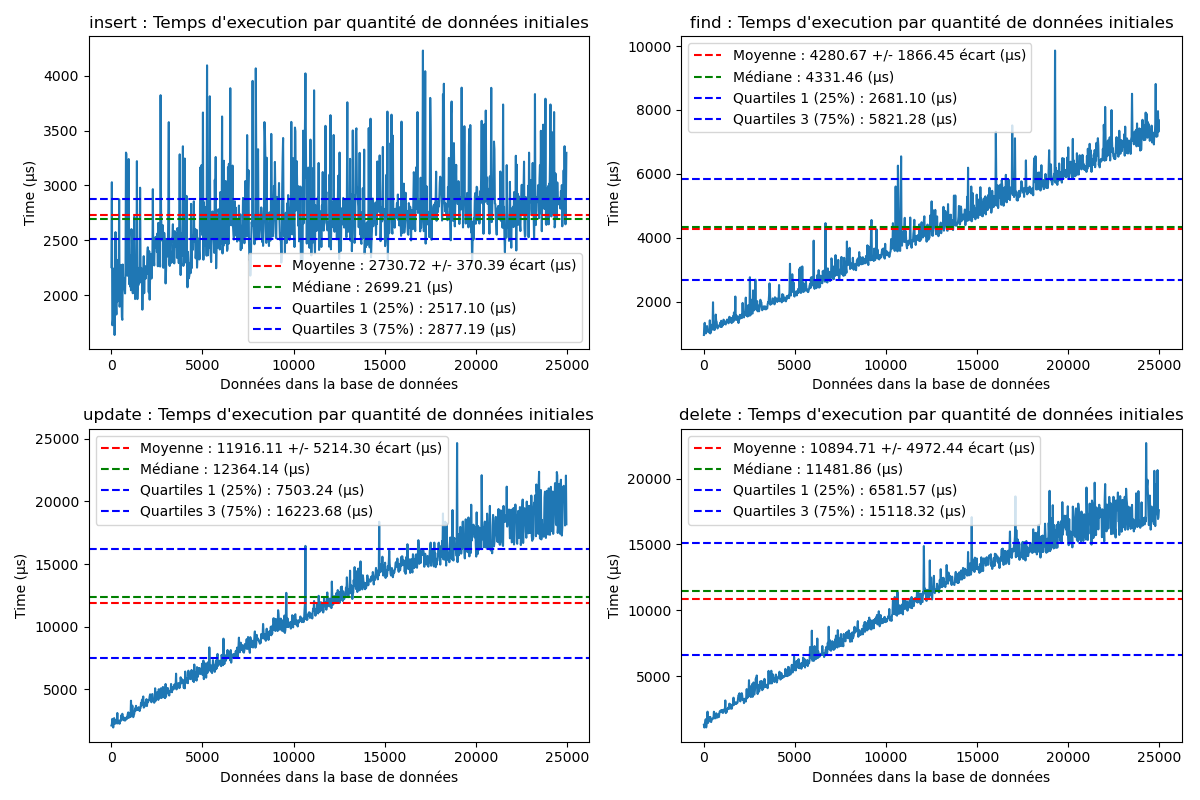
\includegraphics[width=0.8\textwidth]{../plots/MySQL/sharding_indexed/test_many_various_data.png}
                    \caption{Performances des opérations CRUD multiples selon la quantitée de données dans la base.}
                    \label{fig:mysql_cluster_global_many_various_indexed}
                \end{figure}

        \subsection{Observations Globales sur MySQL Cluster} 
            \begin{card}
                Les résultats montrent que MySQL Cluster est plus performant que MySQL Standalone pour les opérations uniques. \\
                Les performances sont comparables à celles de MongoDB, avec des temps d'exécution plus rapides pour les opérations de lecture et de mise à jour. \\
                Les opérations multiples sont plus lentes que les opérations uniques, mais restent plus efficaces pour traiter de grandes quantités de données. \\
                L'indexation améliore les performances des opérations de lecture et de mise à jour, mais a un impact négligeable sur l'insertion et la suppression. \\
                Les performances des opérations CRUD sont plus stables avec l'indexation, ce qui réduit la variance des temps d'exécution. \\
                Enfin, les performances de MySQL Cluster sont comparables à celles de MongoDB en mode standalone. \\
            \end{card}


\chapter{Analyse des Résultats}

\section{Performances des Requêtes}

    \begin{card}
        \begin{itemize}
            \item MongoDB excelle pour les lectures indexées et les mises à jour fréquentes de la structure des données.
            \item MySQL est plus performant pour les requêtes transactionnelles complexes et les lectures indexées.
            \item L'indexation est un facteur clé pour améliorer les performances des requêtes.
            \item Les performances de MongoDB augmentent grandement avec l'indexation.
            \item Paradoxallement, l'indexation n'améliore pas significativement les performances de MySQL.
            \item Les opérations multiples sont plus efficaces pour traiter de grandes quantités de données.
            \item L'indexation permet de stabiliser et d'améliorer le temps d'execution des opérations CRUD.
        \end{itemize}
    \end{card}

\section{Impact de la Réplication et du Sharding}

    \begin{card}
        \begin{itemize}
            \item La réplication et le sharding améliorent la tolérance aux pannes et la scalabilité.
            \item La réplication augmente la latence d'écriture, mais garantit une haute disponibilité des données.
            \item Le sharding améliore les performances des lectures et écritures parallèles par rapport à la réplication.
            \item MySQL Cluster offre des fonctionnalités similaires à MongoDB, mais avec une configuration plus complexe.
            \item MongoDB est plus adapté pour les applications nécessitant une scalabilité horizontale et une haute disponibilité.
        \end{itemize}
    \end{card}

\section{Critique des résultats}

    \begin{card}
        \begin{itemize}
            \item Les tests ont été réalisés sur des configurations de base, sans optimisations spécifiques.
            \item Les performances peuvent varier en fonction de la charge, de la volumétrie des données, et de la configuration matérielle.
            \item Les résultats sont indicatifs et doivent être confirmés par des tests plus approfondis.
            \item Les performances des SGBD dépendent fortement de la nature des requêtes et de la structure des données.
            \item Les tests ont été réalisés sur des scénarios simples, mais les performances peuvent varier dans des cas d'utilisation réels.
        \end{itemize}
    \end{card}

\section{Comparaisons et Bilan}

\begin{table}[h!]
    \centering
    \begin{tabular}{|l|p{7cm}|p{7cm}|}
    \hline
    \textbf{Critère} & \textbf{MongoDB} & \textbf{MySQL} \\ \hline
    Performances CRUD uniques & 
    Stables avec une légère augmentation de la latence pour les données volumineuses. & 
    Performances robustes, mais la latence augmente plus rapidement avec le volume. \\ \hline
    Performances CRUD multiples & 
    Bonne gestion des opérations parallèles, particulièrement avec le sharding. & 
    Dégradation notable des performances avec des données volumineuses. \\ \hline
    Indexation & 
    Impact significatif sur les lectures et mises à jour. Légère pénalité pour les écritures. & 
    Amélioration notable pour les lectures, mais impact moindre sur les mises à jour. \\ \hline
    Réplication & 
    Haute disponibilité avec un impact modéré sur les écritures. & 
    Bonne réplication, mais augmentation notable de la latence des écritures. \\ \hline
    Scalabilité & 
    Scalabilité horizontale efficace grâce au sharding. & 
    Scalabilité plus limitée, dépendante du clustering. \\ \hline
    \end{tabular}
    \caption{Comparaison des performances entre MongoDB et MySQL}
    \label{tab:comparaison_performances}
    \end{table}
    

\chapter{Conclusion}

    \begin{card}
        Cette étude met en évidence les avantages et inconvénients des architectures NoSQL et relationnelles dans divers scénarios. \\
        MongoDB offre une grande flexibilité et scalabilité, totefois, la réplication et le sharding peuvent impacter les performances des opérations CRUD. \\
        Néanmoins, le sharding, s'il est possible est une très bonne solution. \\
        Avec une meilleure configuration, on pourrait s'attendre à des performances similaire au mode standalone et on a tout de même obtenu des meilleures performances que dans le mode répliqué. \\
        Toutefois MySQL, reste performant pour des cas nécessitant des transactions complexes et ne peut montrer l'étendue de ses performances dans un cas aussi simple ne nécessitant pas de modèle relationnel. \\
        De plus, les performances du cluster MySQL s'est avéré, contre toute attente, plus performant que MySQL Standalone, et aussi performante que MongoDB Standalone. \\
    \end{card}

% On crée une partie appendice pour les annexes ou il y a des informations complémentaires, sur le déploiement du code
\appendix
\chapter{Annexe}
\section{Déploiement du Code}


Le projet nécessite l'installation de : 
\begin{itemize}
    \item \href{https://www.python.org/downloads/}{python3}
    \item \href{https://pip.pypa.io/en/stable/installation/}{pip3}
    \item \href{https://docs.docker.com/engine/install/}{docker}
    \item \href{https://docs.docker.com/compose/install/}{docker compose}
\end{itemize}


Ces outils permettent d'installer les dépendances des codes python et de
réaliser les tests de performance de MongoDB et MySQL. Afin de
reproduire les tests de performance, il faut d'abord cloner le dépôt git
suivant:

\begin{card}
    \begin{minted}{bash}
    git clone https://github.com/BJCode-git/Projet-TDLE.git -b main &&
    cd Projet-TDLE
\end{minted}
\end{card}

Il faut ensuite générer les données de test en utilisant les commandes
suivantes:

\begin{card}
    \begin{minted}{bash}
    pip3 install -r requirements/data_generation-requirements.txt &&
    python3 data\_generation.py
\end{minted}
\end{card}

On déploie alors des conteneurs docker pour réaliser des tests de
performance sur une base de données mongodb standalone, une base de
données mongodb répliquée et une base de données mongodb fragmentée.
Pour MySQL, on réalise des tests de performance sur une base de données
standalone et une base de données fragmentée.

Il est possible d'utiliser le script \textbf{start.sh} pour déployer
automatiquement les conteneurs, lancer tous les test puis arrêter les
conteneurs. Cette approche permet de réaliser les tests de performance
de manière automatique et permet de consommer moins de ressources
mémoire et CPU.

\begin{card}
    \begin{minted}{bash}
    chmod +x start.sh &&
    ./start.sh
\end{minted}
\end{card}

Le script \textbf{start.sh} réalise basiquement les opérations
suivantes: - Nettoyage de l'environnement - Crée les dossiers logs et
plots pour les logs et les graphiques - Installation des dépendances
python - Génération des données de test - Test de performance de MongoDB
en standalone - Test de performance de MongoDB en réplication - Test de
performance de MongoDB en sharding - Test de performance de MySQL en
standalone - Test de performance de MySQL en sharding

\emph{Installation des dépendances python :}

\begin{card}
    \begin{minted}{bash}
    pip3 install -r requirements/generate_data-requirements.txt
    pip3 install -r requirements/mongo-requirements.txt
    pip3 install -r requirements/mysql-requirements.txt
\end{minted}
\end{card}

\emph{Génération des données :}

\begin{card}
    \begin{minted}{bash}
    python3 generate_data.py                &&
    docker compose down -v --remove-orphans 
\end{minted}
\end{card}

\subsection{Tests de performance de
MongoDB}

\emph{Test en standalone :}

\begin{card}
    \begin{minted}{bash}
    ## Démarrage et attente de la disponibilité du serveur
    docker compose up mongo-standalone -d --wait &&
    python3 mongodb.py --standalone              &&
    docker compose down -v --remove-orphans
\end{minted}
\end{card}

\emph{Test avec replica :}

\begin{card}
    \begin{minted}{bash}
    docker compose up mongo-replica-initiate &&
    python3 mongodb.py --replica             &&
    docker compose down -v --remove-orphans 
\end{minted}
\end{card}

\emph{Test avec sharding :}

\begin{card}
    \begin{minted}{bash}
    docker compose up mongo-sharded-cluster &&
    python3 mongodb.py --sharded            &&
    docker compose down -v --remove-orphans
\end{minted}
\end{card}

\subsection{Tests de performance de MySQL}

\emph{Test en standalone :}

\begin{card}
    \begin{minted}{bash}
    # Démarrage et attente de la disponibilité du serveur
    docker compose up --wait -d mysql-standalone &&
    python3 mysql.py --standalone                &&
    docker compose down -v --remove-orphans 
\end{minted}
\end{card}

\emph{Test avec sharding :}

\begin{card}
    \begin{minted}{bash}
    docker compose up mysql-sharded-initiate &&
    python3 mysql.py --sharded               &&
    docker compose down -v --remove-orphans
\end{minted}
\end{card}

Il est également possible de séparer les test de performance de MongoDB
et MySQL. Après génération des données, on peut lancer toutes les
infrastructures MongoDB et lancer les tests de performance de MongoDB en
utilisant les commandes suivantes:

\begin{card}
    \begin{minted}{bash}
    docker compose up start_mongo &&
    python3 mongodb.py
    \end{minted}
\end{card}

On peut ensuite stopper les conteneurs docker en utilisant la commande
suivante:

\begin{card}
    \begin{minted}{bash}
    docker compose down -v --remove-orphans
\end{minted}
\end{card}

On peut en faire de même avec MySQL :

\begin{card}
    \begin{minted}{bash}
    docker compose up start_mysql &&
    python3 mysql.py
\end{minted}
\end{card}

Finalement, Pour nettoyer les données générées, on peut utiliser le
script \textbf{clear.sh}:

\begin{card}
    \begin{minted}{bash}
    ./clear.sh
\end{minted}
\end{card}

Note : Il est possible de configurer les paramètres des tests et le
déploiement en modifiant les variables disponibles dans le fichier .env

\end{document}